\documentclass[11pt]{article}
\usepackage[T1]{fontenc}
\usepackage[utf8]{inputenc}
\usepackage{lmodern}
\usepackage[margin=1in]{geometry}
\usepackage{amsmath,amssymb}
\usepackage{graphicx}
\usepackage{xcolor}
\usepackage{booktabs}
\usepackage{multirow}
\usepackage{caption}
\usepackage[most]{tcolorbox}
\usepackage{float}
\usepackage{algorithm}
\usepackage{algorithmic}
\usepackage{hyperref}
\hypersetup{colorlinks=true,linkcolor=blue,citecolor=blue,urlcolor=blue}

% Figures are pulled from the per-comment response folders.
\graphicspath{{../Re1_6/}{../Re1_7/}{../Re2_1/}{../Re2_3/}{../Re2_6/}{../Re3_1/}{../Re3_2/}{../Re3_4/}{../Re3_5/}{../Re3_6/}{../Re3_7/}{../Re3_8/}{../Re3_8/full_v10_asset_truncated/}{../Re3_8/full_v10/}{../Re3_9/}{../HIL_fig/}}

% Colour for text added to the manuscript (matches the blue highlight).
\definecolor{addblue}{RGB}{0,0,205}
\newcommand{\hladd}[1]{{\color{addblue}#1}}

% Verbatim reviewer comment.
\newtcolorbox{reviewercomment}[1]{enhanced,breakable,colback=gray!7,
  colframe=gray!55,boxrule=0.6pt,arc=2pt,left=9pt,right=9pt,top=7pt,bottom=7pt,
  fonttitle=\bfseries,title={#1},coltitle=black,colbacktitle=gray!18,
  fontupper=\itshape}

% Exact text added to the manuscript.
\newtcolorbox{manuscripttext}{enhanced,breakable,colback=blue!4,
  colframe=addblue!55,boxrule=0.6pt,arc=2pt,left=9pt,right=9pt,top=7pt,bottom=7pt}

\newcommand{\rsp}{\medskip\noindent\textbf{Response.}\quad}
\newcommand{\loc}{\medskip\noindent\textbf{Location of the revision.}\quad}
\newcommand{\evi}{\medskip\noindent\textbf{Supporting evidence (this letter).}\quad}

% Two side-by-side sub-panels with bold captions (used by the Re3_8 V10 histories).
% Filenames are resolved through \graphicspath.
\newcommand{\pairedplots}[4]{%
  \begin{minipage}[t]{0.485\textwidth}
    \centering
    \textbf{#1}\par\vspace{1mm}
    \includegraphics[width=\linewidth]{#2}
  \end{minipage}\hfill
  \begin{minipage}[t]{0.485\textwidth}
    \centering
    \textbf{#3}\par\vspace{1mm}
    \includegraphics[width=\linewidth]{#4}
  \end{minipage}\par\vspace{2mm}
}

\title{\vspace{-1.5em}Response to the Reviewers}
\date{}

\begin{document}
\maketitle
\vspace{-3em}
\begin{center}\small
Manuscript: ``Trust-Aware Multi-Agent Reinforcement Learning-Based Cooperative
Interception Strategy for Maneuvering Swarms with Target Assignment''
\end{center}
\bigskip

% \noindent We thank the reviewer for the careful reading and the constructive
% comments. Below, each comment is reproduced verbatim (grey box), followed by our
% point-by-point response, the exact location and wording of the corresponding
% revision in the manuscript (blue box, matching the blue highlight in the revised
% PDF), and the supporting figures prepared for this letter. Equation and section
% numbers refer to the revised manuscript.

\bigskip
\hrule
\bigskip

\section*{Reviewer~1}


% =====================================================================
%  Re1_1
% =====================================================================

\subsection*{Comment 1.1}

\begin{reviewercomment}{Reviewer comment 1.1}
Provide a concise notation table summarizing key variables and symbols used
throughout the paper.
\end{reviewercomment}

\rsp We sincerely thank the reviewer for this helpful suggestion. We agree
that the principal symbols were previously defined across several equations,
making it inconvenient for readers to locate their meanings. We have therefore
added a dedicated appendix entitled ``Summary of Key Variables and Symbols.''

The symbols are organized into three groups corresponding to
the engagement model, IDBO target assignment, and ART-MAPPO cooperative
guidance. The complete addition is reproduced below.

\loc Appendix~A (\emph{Summary of Key Variables and Symbols}), immediately
following the reference list.

\begin{tcolorbox}[enhanced,breakable,colback=white,colframe=addblue!55,
boxrule=0.6pt,arc=2pt,left=9pt,right=9pt,top=7pt,bottom=7pt]
{\color{addblue}

\noindent\textbf{Appendix A: Summary of Key Variables and Symbols}

\medskip
\noindent Table~A summarizes the principal variables and symbols used
throughout the paper.

\medskip
\begin{center}
\textbf{Key Variables and Symbols in Sections II--IV}

\scriptsize
\setlength{\tabcolsep}{2.5pt}
\renewcommand{\arraystretch}{1.10}
\begin{tabular}{@{}p{0.92in}p{1.55in}p{0.92in}p{1.55in}@{}}
\toprule
\textbf{Symbol} & \textbf{Description}
& \textbf{Symbol} & \textbf{Description} \\
\midrule

\multicolumn{4}{@{}l}{\textit{Engagement model}}\\[1pt]

$(x,y,z)$
& UAV position coordinates
& $V,\gamma,\theta$
& Speed, heading, and flight-path angle \\

\shortstack{$\mathbf{p}_A,\mathbf{p}_D$\\
$\mathbf{v}_A,\mathbf{v}_D$}
& Attacker/defender positions and velocities
& $\mathbf{r}_{AD},\boldsymbol{\ell}_{AD}$
& Relative-position vector and LOS unit vector \\

$r,\dot r$
& Relative range and range rate
& $q^\gamma,q^\theta$
& LOS azimuth and elevation \\

$n_x,n_y,n_z$
& Axial, lateral, and normal accelerations
& $t_{go}$
& Estimated time-to-go \\

$\operatorname{ZEM}$
& Zero-effort-miss distance
&
& \\[2pt]

\multicolumn{4}{@{}l}{\textit{IDBO target assignment}}\\[1pt]

$\mathcal{U},\mathcal{T}$
& Interceptor and target sets
& $M,N$
& Numbers of interceptors and targets \\

$X_{ij}$
& Binary assignment of $u_i$ to $t_j$
& $P_{ij}$
& Composite interception probability \\

\shortstack{$w_{1,\mathrm{IDBO}}$\\
$w_{2,\mathrm{IDBO}}$}
& Reachability and geometry weights
& $L_{\max}$
& Per-target interceptor capacity \\

$\mathbf{x}_i$
& Target-preference vector of $u_i$
& $\mathcal{F}_i$
& Local IDBO fitness \\

$A_{ij}$
& Adversarial advantage for pair $(i,j)$
& $\Psi_{ij}$
& Assignment-saturation penalty \\

$\mathcal{N}_i$
& Communication-neighbor set of $u_i$
& \shortstack{$c_{ij}$\\$\mathcal{Z}_j$}
& Bid and winner list for target $t_j$ \\

$c_t$
& Common IDBO decay schedule
& \shortstack{$\Gamma^{(k)}$\\$\epsilon_{\mathrm{IDBO}}$}
& Swarm disagreement and convergence tolerance \\[2pt]

\multicolumn{4}{@{}l}{\textit{ART-MAPPO cooperative guidance}}\\[1pt]

$\mathbf{o}_i^{(t)}$
& Local observation of interceptor $i$
& $s_t$
& Centralized global state \\

$\mathbf{A}_j$
& Attention matrix of head $j$
& $\mathbf{c}_t$
& GRU hidden state \\

$\pi_{\boldsymbol{\vartheta}_i}$
& Decentralized actor policy
& $V_\phi(s_t)$
& Centralized critic value \\

$\mathbf{a}_i$
& Three-axis acceleration command
& $\mathcal{T}_i^{(k)}$
& Smoothed trust level \\

$\tilde{R}_i^{(k)}$
& Normalized relative return
& \shortstack{$\beta(\mathcal{T}_i)$\\
$\pi_{\mathrm{guided}}^i$}
& Guided-policy weight and distribution \\

$\hat{A}_t$
& GAE advantage estimate
& \shortstack{$r_t(\boldsymbol{\vartheta})$\\$\epsilon$}
& Probability ratio and PPO clip threshold \\

$J^{\mathrm{DC}},c$
& Dual-Clip objective and floor
& \shortstack{$\hat{D}_{\mathrm{KL}}$\\
$\beta_{\mathrm{KL}},\delta_{\mathrm{targ}}$}
& KL estimate, penalty coefficient, and target \\

$r_i^{(t)}$
& Per-step composite reward
& $w_1,\ldots,w_5$
& Reward-component weights \\

$\mathcal{G}_i$
& Same-target interceptor group
& $\bar{t}_{go}^{(t)}$
& Group mean time-to-go \\

$L_V(\phi)$
& Centralized critic value loss
& $\mathcal{L}(\boldsymbol{\vartheta},\phi)$
& Overall training loss \\

\bottomrule
\end{tabular}
\end{center}
}
\end{tcolorbox}



% =====================================================================
%  Re1_2
% =====================================================================


\subsection*{Comment 1.2}

\begin{reviewercomment}{Reviewer comment 1.2}
Include pseudocode or algorithm boxes for IDBO and ART-MAPPO to improve
reproducibility.
\end{reviewercomment}

\rsp We sincerely thank the reviewer for this valuable suggestion. We agree
that the equations in the original manuscript defined the individual
components of IDBO and ART-MAPPO, but did not provide sufficiently compact
procedural descriptions for reproducing the complete algorithms. We have
therefore added two pseudocode boxes to the revised manuscript.

Algorithm~1 summarizes the complete distributed IDBO assignment procedure,
including local candidate generation, fitness evaluation, preference
thresholding, bid exchange, conflict resolution, and the consensus stopping
criterion. Algorithm~2 presents the ART-MAPPO training procedure under the
CTDE paradigm, covering decentralized rollout collection, trust updating,
advantage estimation, centralized actor--critic optimization, and adaptive
KL regulation. The steps in both algorithms are cross-referenced to their
governing equations in the revised manuscript. The two added algorithms are
reproduced below for the reviewer's convenience.

\medskip
\noindent\textbf{(1) IDBO target-assignment pseudocode.}

\loc Section~III-B (\emph{Distributed Consensus-Based IDBO Framework}),
immediately after the convergence criterion in Eq.~(26) and before the
per-UAV complexity analysis in Eq.~(27).

\begin{tcolorbox}[enhanced,breakable,colback=white,colframe=addblue!55,
boxrule=0.6pt,arc=2pt,left=9pt,right=9pt,top=7pt,bottom=7pt]
{\color{addblue}
\noindent\textbf{Algorithm 1: IDBO Target Assignment}

\medskip
\begin{algorithmic}[1]
\REQUIRE Interceptor and target sets $\mathcal{U},\mathcal{T}$;
engagement states; communication graph; capacity $L_{\max}$;
local population size $N_{\mathrm{pop}}$; local search horizon $T$;
tolerance $\epsilon_{\mathrm{IDBO}}$

\ENSURE Feasible consensus assignment $\mathbf{X}^{\ast}$

\STATE Each interceptor $u_i$ initializes a local preference population,
assignment replica, bid/winner records, and timestamps;
set $k\!\leftarrow\!0$

\REPEAT

  \STATE Evaluate $\mathbf{P}$ using Eq.~(8) and the adversarial
  advantages using Eq.~(15)

  \FOR{$t=1$ to $T$}

    \STATE Set the linearly decaying coefficients
    $c_t=c_0(1-t/T)$ for the four IDBO operators

    \STATE Evaluate all local candidates with
    $\mathcal{F}_i$ in Eq.~(13)

    \STATE Generate candidates using the rolling, dancing, breeding,
    and stealing operators according to Eqs.~(16)--(19)

  \ENDFOR

  \STATE Select and binarize the best local preference using Eq.~(20);
  compute the target bids using Eq.~(21)

  \STATE Exchange local records with $\mathcal{N}_i$, update the
  top-$L_{\max}$ winner lists using Eq.~(22), and resolve assignment
  conflicts subject to the constraints in Eq.~(11)

  \STATE Update the local feasible assignment replica and adversarial
  information; evaluate consensus disagreement;
  $k\!\leftarrow\!k+1$

\UNTIL{the disagreement falls below $\epsilon_{\mathrm{IDBO}}$}

\STATE Set $\mathbf{X}^{\ast}$ to the common feasible assignment replica

\STATE \textbf{return} $\mathbf{X}^{\ast}$

\end{algorithmic}
}
\end{tcolorbox}

\medskip
\noindent\textbf{(2) ART-MAPPO training pseudocode.}

\loc Section~IV-C (\emph{Robust Optimization via Dual-Clip and Adaptive
KL}), immediately after the ART-MAPPO workflow in Fig.~5 and before
Section~IV-D (\emph{Mechanistic Comparison with Conventional MAPPO}).

\begin{tcolorbox}[enhanced,breakable,colback=white,colframe=addblue!55,
boxrule=0.6pt,arc=2pt,left=9pt,right=9pt,top=7pt,bottom=7pt]
{\color{addblue}
\noindent\textbf{Algorithm 2: ART-MAPPO for Cooperative Swarm Interception}

\medskip
\begin{algorithmic}[1]

\REQUIRE Actor parameters
$\{\boldsymbol{\vartheta}_i\}_{i=1}^{M}$;
centralized critic parameters $\phi$; episode horizon $T$;
training episodes $K$; PPO clip parameter $\epsilon$;
dual-clip floor $c$; target KL divergence $\delta_{\mathrm{targ}}$;
trust parameters $\alpha_T$, $\rho$, and $\tau_T$;
optimizer parameters

\ENSURE Trained decentralized policies
$\{\pi_{\boldsymbol{\vartheta}_i}\}_{i=1}^{M}$

\STATE Initialize $\{\boldsymbol{\vartheta}_i\}_{i=1}^{M}$ and $\phi$;
set $\mathcal{T}_i\leftarrow0.5$ for each interceptor;
initialize $\beta_{\mathrm{KL}}$ and the running return statistics
$\mu_R$ and $\sigma_R^2$

\FOR{episode $k=1$ to $K$}

  \STATE Reset the environment, clear the rollout buffer,
  and reset $\mathbf{c}_{i,0}$ for each interceptor

  \STATE Set
  $\boldsymbol{\vartheta}_{i,\mathrm{old}}
  \leftarrow\boldsymbol{\vartheta}_i$
  for all $i=1,\ldots,M$

  \STATE {\itshape // Decentralized rollout collection}

  \FOR{$t=0$ to $T-1$}

    \FOR{all interceptors $i=1,\ldots,M$ in parallel}

      \STATE Encode $\mathbf{o}_i^{(t)}$ using the attention--residual
      network according to Eqs.~(28)--(34), and update the temporal state
      $\mathbf{c}_{i,t}$ using the GRU in Eq.~(36)

      \STATE Form the policy
      $\pi_{\boldsymbol{\vartheta}_i}
      (\cdot\mid\mathbf{o}_i^{(t)})$
      according to Eq.~(37), and sample $\mathbf{a}_{i,t}$
      according to Eqs.~(43)--(44), with
      $\beta(\mathcal{T}_i)=1-\mathcal{T}_i$

      \STATE Clip $\mathbf{a}_{i,t}$ to the three-dimensional feasible
      action envelope $\mathcal{A}$

    \ENDFOR

    \STATE Step the environment once using the joint action
    $\mathbf{a}_t=(\mathbf{a}_{1,t},\ldots,\mathbf{a}_{M,t})$
    and store the joint transition in the rollout buffer

  \ENDFOR

  \STATE {\itshape // Trust update based on episode returns}

  \STATE Update $\mu_R$ and $\sigma_R^2$ using Eqs.~(39)--(40),
  and compute the normalized return $\widetilde{R}_i^{(k)}$
  using Eq.~(41)

  \STATE Update the trust level
  $\mathcal{T}_i^{(k+1)}$ using Eq.~(42)

  \STATE {\itshape // Centralized optimization using the global state
  defined in Eq.~(38)}

  \STATE Compute the GAE advantages $\hat{A}_t$ and value targets
  using Eqs.~(46)--(47)

  \FOR{each mini-batch update}

    \STATE Evaluate the dual-clip surrogate objective
    $J^{\mathrm{DC}}(\boldsymbol{\vartheta})$
    using Eqs.~(48)--(49)

    \STATE Estimate $\widehat{D}_{\mathrm{KL}}$ using Eq.~(51),
    and compute the value loss $L_V(\phi)$ using Eq.~(53)

    \STATE Update $\{\boldsymbol{\vartheta}_i\}_{i=1}^{M}$ and $\phi$
    by minimizing the total loss
    $\mathcal{L}(\boldsymbol{\vartheta},\phi)$ in Eq.~(54)
    using AdamW with cosine learning-rate scheduling

  \ENDFOR

  \STATE Adapt the KL weight
  $\beta_{\mathrm{KL}}^{(k+1)}$ using Eq.~(52)

\ENDFOR

\STATE \textbf{return}
$\{\pi_{\boldsymbol{\vartheta}_i}\}_{i=1}^{M}$

\end{algorithmic}
}
\end{tcolorbox}



% =====================================================================
%  Re1_3
% =====================================================================
\subsection*{Comment 1.3}

\begin{reviewercomment}{Reviewer comment 1.3}
Add intuitive explanations before or alongside major equations, especially
in Sections III and IV.
\end{reviewercomment}

\rsp We sincerely thank the reviewer for this careful and constructive
suggestion. We agree that, although the major equations in Sections~III and
IV were mathematically defined, the original manuscript left some of their
algorithmic and physical meanings implicit. This could make it difficult for
readers to connect the mathematical operations with the corresponding target
assignment and policy-learning processes. We have therefore added concise
explanations immediately alongside eight groups of major equations. These
revisions clarify the roles of the principal terms, the flow of information
between successive operations, and their effects on the proposed framework.
The equation numbers below refer to the revised manuscript. The corresponding
additions are reproduced in blue in the white boxes.

\medskip
\noindent\textbf{(1) IDBO fitness function and saturation penalty.}

\loc Section~III-B (\emph{Distributed Consensus-Based IDBO Framework}),
immediately after Eqs.~(14)--(15). We added an intuitive interpretation of
how the fitness function combines target preference with the saturation
penalty.

\begin{tcolorbox}[enhanced,breakable,colback=white,colframe=addblue!55,
boxrule=0.6pt,arc=2pt,left=9pt,right=9pt,top=7pt,bottom=7pt]
\hladd{In intuitive terms, each interceptor increases its preference
for targets that combine high interception likelihood with a strong
tactical advantage, while the saturation penalty redirects the local search
when neighboring preferences indicate that a target has reached its
allocation capacity.}
\end{tcolorbox}

\medskip
\noindent\textbf{(2) Three-dimensional geometric term in the adversarial
advantage.}

\loc Section~III-B, in Eq.~(15) and the paragraph immediately following it.
The geometric factor is expressed through the normalized inner product
between the interceptor velocity and the target LOS, and its physical
meaning in the three-dimensional engagement is stated explicitly.

\begin{tcolorbox}[enhanced,breakable,colback=white,colframe=addblue!55,
boxrule=0.6pt,arc=2pt,left=9pt,right=9pt,top=7pt,bottom=7pt]
\begin{equation*}
\begin{split}
A_{ij} =&
\exp\left(-\frac{\Delta t_{ij}}{T_{\max}}\right)
\left(1-\frac{\|\mathbf{v}_i-\mathbf{v}_j\|_2}{v_{\max}}\right) \\
&\cdot
\hladd{\max\left(0,
\frac{\mathbf{v}_i^{\top}(\mathbf{p}_j-\mathbf{p}_i)}
{\|\mathbf{v}_i\|_2\,\|\mathbf{p}_j-\mathbf{p}_i\|_2}\right)} \\
&-\sum_{k\neq i}\frac{P_{kj}}{P_{ij}+P_{kj}}
\cdot\sigma(\hat{x}_{kj}).
\end{split}
\end{equation*}

\hladd{$\mathbf{p}_i=[x_i,y_i,z_i]^\top$ and
$\mathbf{v}_i=[\dot{x}_i,\dot{y}_i,\dot{z}_i]^\top$ denote the
three-dimensional position and velocity vectors of interceptor $u_i$, while
$\mathbf{p}_j=[x_j,y_j,z_j]^\top$ and
$\mathbf{v}_j=[\dot{x}_j,\dot{y}_j,\dot{z}_j]^\top$ denote those of target
$t_j$.}

\medskip
\hladd{The normalized inner product is the cosine of the three-dimensional
angle between the interceptor velocity and the LOS to target $t_j$; the
maximum operator assigns zero geometric advantage when the target lies
outside the interceptor's forward hemisphere.}
\end{tcolorbox}

\medskip
\noindent\textbf{(3) Decay mechanism of the four IDBO update operators.}

\loc Section~III-B, immediately after the rolling, dancing, breeding, and
stealing operators in Eqs.~(16)--(19), and before the thresholding equation.
We explained how the decaying coefficients progressively suppress the
stochastic components of the four update operators.

\begin{tcolorbox}[enhanced,breakable,colback=white,colframe=addblue!55,
boxrule=0.6pt,arc=2pt,left=9pt,right=9pt,top=7pt,bottom=7pt]
\hladd{The coefficients
$\alpha,\beta,\gamma_{\mathrm{IDBO}},\delta,\delta',
\eta_{\mathrm{IDBO}}$ together with the dancing noise scale $\sigma_d$
follow a common linear schedule $c_t=c_0\,(1-t/T)$, where $T$ is the IDBO
iteration count, while the elite-recombination weights remain bounded. This
schedule is what governs convergence stability. The stochastic parts of the
operators---the rolling probe
$\beta\,\boldsymbol{\xi}_i\mathrm{e}^{-t/T}$ and the dancing perturbation
$\mathbf{n}_i\sim\mathcal{N}(0,\sigma_d^2\mathbf{I})$---scale with $c_t$ and
vanish as $c_t\!\to\!0$, so the update degenerates into a deterministic,
advantage-weighted local refinement followed by the advantage-adaptive
binarization step. A step sequence whose stochastic amplitude decays to zero
while retaining an ascent direction satisfies a Robbins--Monro-type
sufficient condition for settling at a stable fixed point rather than
orbiting it, which is precisely the behavior measured by the
swarm-disagreement metric $\Gamma^{(k)}$ in Eq.~(30). A controlled ablation
that freezes the coefficients confirms this mechanism: non-decaying
coefficients keep injecting perturbations and leave a persistent late-stage
oscillation in the working assignment, whereas the linear schedule contracts
the swarm onto a stable, low-cost equilibrium.}
\end{tcolorbox}

\medskip
\noindent\textbf{(4) Thresholding, bidding, and neighborhood-consensus
updates.}

\loc Section~III-B, immediately after the neighborhood-consensus update in
Eq.~(22). We added a concise explanation connecting the thresholding,
bidding, and winner-list updates in Eqs.~(20)--(22).

\begin{tcolorbox}[enhanced,breakable,colback=white,colframe=addblue!55,
boxrule=0.6pt,arc=2pt,left=9pt,right=9pt,top=7pt,bottom=7pt]
\hladd{Equations~(20)--(22) convert the continuous preferences into local
assignment candidates. Their bids are exchanged among neighboring
interceptors so that at most the $L_{\max}$ strongest candidates are retained
for each target, and repeated exchanges bring the local winner lists into
agreement.}
\end{tcolorbox}

\medskip
\noindent\textbf{(5) Attention matrix and output projection.}

\loc Section~IV-A (\emph{Enhanced Situational Awareness via
Attention-Residual Network}), immediately after the multi-head attention
output in Eq.~(31). We clarified the interpretation of the attention matrix
in Eq.~(30) and the role of the output projection in Eq.~(31).

\begin{tcolorbox}[enhanced,breakable,colback=white,colframe=addblue!55,
boxrule=0.6pt,arc=2pt,left=9pt,right=9pt,top=7pt,bottom=7pt]
\hladd{Each row of $\mathbf{A}_j$ specifies how the observable
kinematic features contribute to the update of one feature token. After the
head outputs are concatenated and flattened, $\mathbf{W}^{O}$ maps the
attended information from all feature tokens back to the $d$-dimensional
latent space for residual fusion with $\mathbf{h}^{(0)}$.}
\end{tcolorbox}

\medskip
\noindent\textbf{(6) Two information paths in the residual block.}

\loc Section~IV-A, immediately after the residual-block updates in
Eqs.~(32)--(34), and before the Jacobian analysis in Eq.~(35). We explained
the distinct functions of the nonlinear branch and the identity shortcut.

\begin{tcolorbox}[enhanced,breakable,colback=white,colframe=addblue!55,
boxrule=0.6pt,arc=2pt,left=9pt,right=9pt,top=7pt,bottom=7pt]
\hladd{The nonlinear branch refines the attended representation, while
the shortcut carries the incoming engagement features directly to the next
block. This structure reduces the need to reconstruct unchanged kinematic
information at every layer.}
\end{tcolorbox}

\medskip
\noindent\textbf{(7) Smoothing process of the trust update.}

\loc Section~IV-B (\emph{Trust-Modulated Tactical Exploration}),
immediately after the trust update in Eq.~(42). We added an intuitive
explanation of the bounded performance reference, the smoothing operation,
and the resulting adjustment of exploration.

\begin{tcolorbox}[enhanced,breakable,colback=white,colframe=addblue!55,
boxrule=0.6pt,arc=2pt,left=9pt,right=9pt,top=7pt,bottom=7pt]
\hladd{The sigmoid term maps the normalized relative return
$\tilde{R}_i^{(k)}$ to a bounded performance reference in $(0,1)$.
Equation~(42) combines the previous trust level and the current performance
reference with the weights $1-\alpha_T$ and $\alpha_T$, respectively,
yielding a smoothed trust estimate. The smoothing process tracks changes in
relative performance while attenuating episode-to-episode return
fluctuations. Sustained above-average returns keep the performance reference
above $0.5$ and bias the smoothed trust estimate toward a correspondingly
higher level, thereby reducing the probability assigned to the guided
exploratory policy; sustained below-average returns produce the opposite
allocation.}
\end{tcolorbox}

\medskip
\noindent\textbf{(8) Overall ART-MAPPO loss function.}

\loc Section~IV-C (\emph{Robust Optimization via Dual-Clip and Adaptive
KL}), immediately after the overall loss in Eq.~(54). We clarified which
loss terms update the actor and critic and how the remaining terms regulate
policy change and exploration.

\begin{tcolorbox}[enhanced,breakable,colback=white,colframe=addblue!55,
boxrule=0.6pt,arc=2pt,left=9pt,right=9pt,top=7pt,bottom=7pt]
\hladd{Minimizing this loss updates the actor through the Dual-Clip
objective, while the KL and entropy terms regulate policy change and
exploration. The value-loss term trains the centralized critic.}
\end{tcolorbox}

% \medskip
% \noindent Collectively, these additions place the requested intuition
% directly alongside the corresponding mathematical definitions in
% Sections~III and IV, allowing the assignment and policy-learning procedures
% to be followed without relying on explanations provided later in the
% manuscript.


% =====================================================================
%  Re1_4
% =====================================================================
\subsection*{Comment 1.4}

\begin{reviewercomment}{Reviewer comment 1.4}
Expand discussion on real-world applicability, including communication delays,
sensing uncertainty, and 3D dynamics.
\end{reviewercomment}

\rsp We thank the reviewer for this suggestion, which we have addressed structurally
rather than as an added paragraph. The revised evaluation is now conducted in a full
\emph{three-dimensional} engagement, and the three factors the reviewer lists are
built into the closed loop rather than discussed in the abstract:
\begin{itemize}
  \item \textbf{3D dynamics.} The kinematic and line-of-sight models in Section~II are
  extended from the planar formulation to three dimensions. A pitch (flight-path)
  channel and its associated normal load $n_z$ are added, the velocity is resolved
  into $(\dot x,\dot y,\dot z)$ through the pitch and heading angles, and the
  zero-effort-miss and relative-geometry relations are rewritten in vector form. The
  original planar definitions are preserved as the horizontal projection, so the
  extension supplements rather than replaces the established notation.
  \item \textbf{Communication delay.} A sensing delay of $100$~ms and a command-channel
  delay of $50$~ms are injected as explicit delay lines in the evaluation (new
  Communication-Delay and Observation-Uncertainty table in Section~V); its effect on the
  distributed IDBO consensus is quantified directly below and analyzed in full in
  Comment~3.2.
  \item \textbf{Sensing uncertainty.} Zero-mean Gaussian position ($\sigma_p=3$~m) and
  velocity ($\sigma_v=0.3$~m/s) errors are added to every observation; a dedicated
  robustness study (Comment~3.7) quantifies the guidance loop's tolerance.
\end{itemize}

To make the communication-delay point concrete, we sweep the per-link delay $\tau$ on the
paper's engagement (40 defenders, 12 targets) and measure the time for the distributed
consensus to reach and hold full agreement ($\Gamma\!\to\!0$):

\begin{table}[h]
\centering
\captionsetup{font=small}
\caption*{\small Distributed-consensus time vs.\ communication delay (40 vs.\ 12
engagement; nominal $20$~Hz link).}
\begin{tabular}{lcccccc}
\toprule
Communication delay $\tau$ (ms) & 0 & 50 & 100 & 200 & 400 & 800 \\
\midrule
Time to consensus (s) & 0.57 & 0.90 & 1.23 & 1.88 & 3.08 & 5.54 \\
\bottomrule
\end{tabular}
\end{table}

\noindent Every setting still reaches full consensus; the delay changes neither the fixed
point nor the correctness, only the speed, with the consensus time growing linearly in the
delay. A representative $20$~Hz link ($\tau=50$~ms) settles the assignment in under $1$~s,
so real-world communication delay is tolerated rather than merely discussed. The full
complexity, scalability, and diameter analysis is given in Comment~3.2.

These are demonstrated on a hardware-in-the-loop, semi-physical platform (Comment~3.10),
so ``real-world applicability'' is shown empirically.

\loc Section~II (3D kinematics, LOS geometry, loads, and ZEM equations, all highlighted
in blue); Section~V-A (\emph{Experimental Setup and Implementation Details}): the
communication-delay and observation-uncertainty model , the HIL
platform description.
% and a closing paragraph quantifying graceful degradation under
% quadrupled noise, $20\%$ packet loss, and $10\%$ per-unit interceptor failure. Detailed
% supporting material is in the response folder for this comment.

\clearpage

% =====================================================================
%  Re1_5
% =====================================================================
\subsection*{Comment 1.5}

\begin{reviewercomment}{Reviewer comment 1.5}
Discuss the sensitivity of the reward function with respect to weights and
hyperparameters.
\end{reviewercomment}

\rsp We thank the reviewer and address the two axes of this sensitivity separately: the
\emph{reward weights} of Eq.~(66), which shape the learning objective, and the
\emph{training hyperparameters} of Table~I, which govern the optimizer. Both are now
treated in the new sensitivity subsection, Section~V-G (\emph{Parameter Sensitivity
Analysis}).

\medskip\noindent\textbf{1) Reward weights (objective shaping).} As detailed in our reply
to Comment~3.5 and in Section~V-G-2) / Table~VII, a one-at-a-time perturbation of the five
reward weights $w_1$--$w_5$---each scaled by $s\in\{0.50,0.75,1.00,1.25,1.50\}$ with the
policy retrained and re-evaluated at every setting---shows that each weight primarily
shapes its intended tactical dimension: $w_4$ governs temporal coordination
($E_{co\text{-}time}$ swings $\approx55\%$), $w_5$ governs terminal overload $E_n$, $w_1$
governs terminal precision $E_{miss}$, and $w_3$ governs reliability (ISR). Across the
entire sweep the interception success rate stays high ($\geq96.2\%$ except for the
strongly under-weighted terminal-hit case), so the shaping weights are tactical dials
rather than knife-edges on effectiveness. We do not restate the full metric table here to
avoid duplicating Comment~3.5.

\medskip\noindent\textbf{2) Training hyperparameters (optimizer).} We conducted a
one-at-a-time (OAT) sensitivity study over the three principal optimization
hyperparameters---the initial learning rate $\eta_0$, the PPO clipping factor $\epsilon$,
and the adaptive-KL target $\delta_{\text{targ}}$. Each parameter is swept over five values
while the others are held at their nominal settings (listed with their optimization roles in
Table~I), and the policy is retrained under the same training budget for every
configuration. We report the training AUC (area under the normalized-reward curve, in units
of $10^4$) and the final normalized reward (averaged over the last $500$ episodes) in the
new Table~VIII (manuscript Section~V-G-3)). The learning rate has the strongest influence:
moving $\eta_0$ from the nominal $3\times10^{-4}$ to $1\times10^{-3}$ lowers the training AUC
and final reward by $13.9\%$ and $5.8\%$, whereas the neighboring value $2\times10^{-4}$
changes them by only $3.3\%$ and $0.3\%$. The clipping factor is essentially flat over
$\epsilon\in[0.15,0.25]$ (variations $\leq\!0.60\%$ in AUC and $\leq\!0.31\%$ in final reward
relative to nominal), and $\delta_{\text{targ}}=0.02$ balances training efficiency against
converged performance (raising it to $0.04$ costs $5.63\%$ AUC and $2.57\%$ final reward).
These results show the nominal configuration sits within a stable high-performance
neighborhood rather than at an isolated favorable point.

\medskip\noindent This is corroborated by the five-seed training study (Section~V-C,
Fig.~11): at the nominal configuration, five independently-initialized runs converge to an
asymptotic normalized reward of $8.97\pm0.64$ (mean\,$\pm$\,std over the final $500$
episodes), a cross-seed standard deviation ($\sigma=0.64$) about half that of standard MAPPO
($\sigma=1.34$), reaching $90\%$ of peak performance by episode~$5{,}591$.

\medskip\noindent The dual-clip surrogate and adaptive-KL penalty are presented in
Section~IV as designed: the dual-clip bound keeps the policy ratio within
$[1/c,c]$ under negative advantage, and the adaptive-KL term regulates the per-update
policy shift toward $\delta_{\text{targ}}$. We describe these as the mechanisms that keep
each update well-conditioned; we do not claim they render the outcome independent of every
hyperparameter, and the OAT sweep and multi-seed evidence above are what substantiate the
robustness claim.

\loc Section~V-G (\emph{Parameter Sensitivity Analysis}): part~2) (reward-weight
sensitivity, Table~VII) and part~3) (training-hyperparameter robustness, new Table~VIII OAT
sweep, corroborated by the five-seed study of Section~V-C / Fig.~11). Table~I has been
extended with a ``Role in optimization'' column listing each hyperparameter for this comment.



\subsection*{Comment 1.6 }

\begin{reviewercomment}{Reviewer comment 1.6}
Provide rigorous discussion on the convergence claims and equilibrium properties.
\end{reviewercomment}

\rsp We thank the reviewer for this important point. In the original manuscript the
convergence and equilibrium statements were asserted without stating their assumptions or
their governing results, and two of them were phrased more strongly than what the method
actually guarantees. We have made each claim precise: we now state the conditions under
which it holds, name the established result it rests on with a proper citation, and---where
the original wording overreached---scope it down to the honest guarantee. The revision
spans both the assignment layer (IDBO) and the guidance layer (ART-MAPPO). Table~R6
summarizes the before/after of every claim, and a new figure confirms the two IDBO
properties on the exact quantities they concern.

\medskip\noindent\textbf{1) Target assignment (IDBO).} The single sentence that previously
bundled three assertions is replaced by three separately-justified statements under
explicit assumptions (connected communication graph of diameter $D$, bounded message delay,
elitist retention):
\begin{itemize}
  \item \emph{Monotonicity.} We now claim monotonicity of the \emph{incumbent}
  (best-so-far) fitness $\Phi_{\mathrm{best}}^{(k)}$, which holds by construction under
  elitism. The original ``$\Phi^{(k+1)}\!\ge\!\Phi^{(k)}$ almost surely'' for the working
  population was not correct while the stochastic operators are active; the decaying
  coefficient schedule $c_t=c_0(1-t/T)$ then drives the operator noise to zero, giving the
  Robbins--Monro condition for stochastic-approximation convergence to a fixed point.
  \item \emph{Consensus time.} The ``at most $N\!\cdot\!D$ iterations'' claim is precisely
  the guarantee of the consensus-based bundle algorithm (CBBA) under a diminishing-marginal-gain
  (submodular) score; we now attribute it accordingly rather than asserting it bare.
  \item \emph{Equilibrium.} We replace ``$\epsilon$-approximate Nash equilibrium'' with
  ``$\epsilon$-\emph{stable} assignment.'' The two describe the same condition (no
  interceptor gains more than $\epsilon$ by a unilateral reassignment), but ``Nash'' would
  require formally defining the underlying game; ``$\epsilon$-stable'' states exactly what
  the auction best-response at the converged bid prices delivers, without that overhead.
\end{itemize}

\medskip\noindent\textbf{2) Cooperative guidance (ART-MAPPO).} Two claims are made rigorous:
\begin{itemize}
  \item \emph{Trust dynamics.} The trust update Eq.~(46) is a first-order exponential-smoothing
  map: for $\alpha_T\in(0,1)$ it combines the previous trust level with a bounded performance
  reference $\sigma(\tau_T\tilde R_i)\in(0,1)$, so trust stays in $(0,1)$ and tracks that
  bounded reference rather than accumulating. The revised manuscript now states this
  bounded-smoothing behavior explicitly; the underlying contraction of modulus $(1-\alpha_T)$
  is elementary and is derived in our response to Comment~2.3.
  \item \emph{Policy convergence.} The original text claimed the dual-clip bound makes the
  ``monotonic-improvement/stationary-point guarantees of trust-region policy optimization
  carry over.'' We scope this to the honest ceiling for any PPO-family method: the bounded
  ratio $r_t\in[1/c,c]$ gives a Lipschitz-bounded surrogate gradient, hence convergence to
  an $\epsilon$-\emph{stationary point of the KL-penalized surrogate} under the standard
  nonconvex stochastic-approximation conditions---not to a global optimum and not a monotone
  improvement of the true return. Trust-region policy optimization is cited as the principle
  that \emph{motivates} the bounded-shift design, not as a guarantee inherited verbatim.
\end{itemize}

\medskip\noindent Four references now anchor these results: CBBA for the distributed-consensus
guarantee, trust-region policy optimization for the bounded-policy-shift principle, and the
Robbins--Monro and nonconvex stochastic-approximation results for the fixed-point/stationary-point
convergence. None were cited in the original manuscript.

\evi Fig.~R23 confirms the two IDBO properties on the exact quantities they concern, using
the paper's own engagement scenario. Panel~(a) shows the swarm-disagreement metric
$\Gamma^{(k)}$ of Eq.~(30): with the proposed linear-decay schedule it settles below the
convergence threshold ($\Gamma_{\text{final}}\!=\!0.004$) and holds there, whereas constant or
non-decaying coefficients leave it oscillating an order of magnitude higher
($0.036$ and $0.048$)---the direct measurement behind the ``settles at a fixed point rather
than orbiting it'' statement. Panel~(b) shows that the number of consensus rounds grows
near-linearly with the communication-graph diameter $D$ (about $4.6$ rounds per unit $D$),
empirically confirming the $O(N\!\cdot\!D)$ bound.

\begin{figure}[h]
\centering
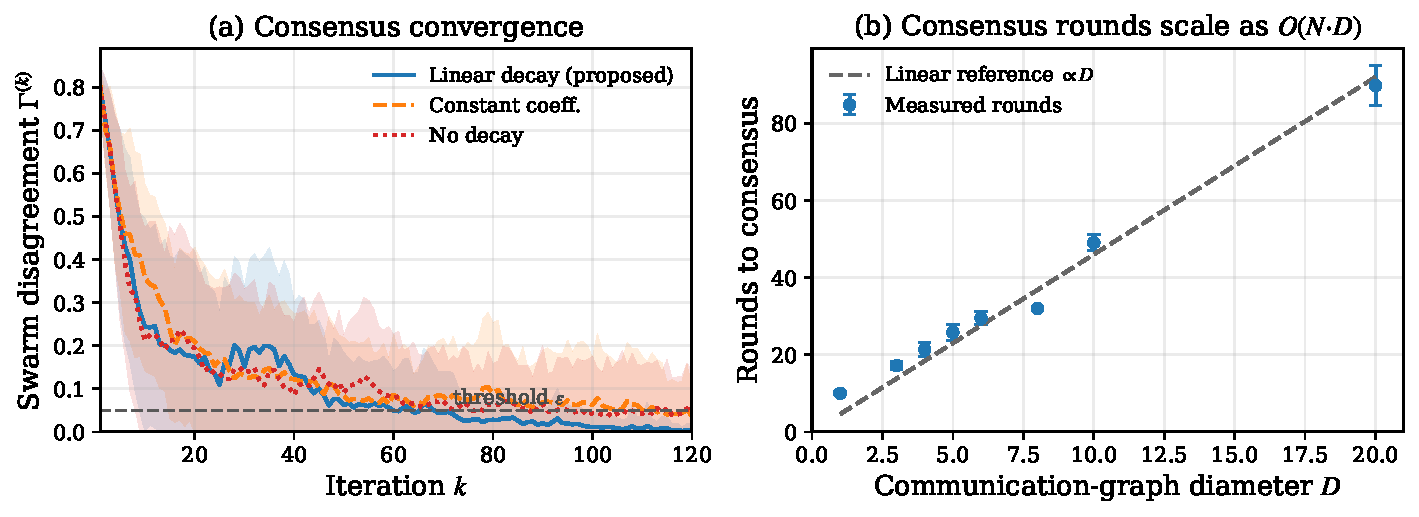
\includegraphics[width=\textwidth]{re1_7_convergence.pdf}
\captionsetup{font=small}
\caption*{\small\textbf{Fig.~R23.} Empirical confirmation of the IDBO convergence claims.
\textbf{(a)} Swarm-disagreement metric $\Gamma^{(k)}$ [Eq.~(30)] versus iteration for the
three coefficient schedules ($40$ runs each; mean $\pm$ std). The proposed linear-decay
schedule drives $\Gamma^{(k)}$ below the convergence threshold $\epsilon$ and holds it there,
while constant and no-decay coefficients keep it oscillating an order of magnitude higher.
\textbf{(b)} Rounds to consensus versus communication-graph diameter $D$; the near-linear
growth confirms the $O(N\!\cdot\!D)$ bound established for the consensus-based bundle
algorithm.}
\end{figure}

\begin{table}[h]
\centering
\caption*{\small\textbf{Table~R6.} Convergence/equilibrium claims: original wording vs.\ the
rigorous revised statement, with the governing result now cited.}
\renewcommand{\arraystretch}{1.3}
\footnotesize
\begin{tabular}{@{}p{0.16\textwidth} p{0.34\textwidth} p{0.34\textwidth}@{}}
\toprule
\textbf{Claim} & \textbf{Original (asserted, uncited)} & \textbf{Revised (rigorous, cited)}\\
\midrule
IDBO monotonicity & $\Phi^{(k+1)}\!\ge\!\Phi^{(k)}$ a.s.\ (working population) & Incumbent (best-so-far) $\Phi_{\mathrm{best}}^{(k)}$ non-decreasing under elitism; fixed point via Robbins--Monro decay [Robbins--Monro]\\
IDBO consensus & Consensus in $\le N\!\cdot\!D$ iterations & Same bound, attributed to CBBA under submodular scoring [Choi--Brunet--How]\\
IDBO equilibrium & $\epsilon$-approximate Nash equilibrium & $\epsilon$-stable assignment (auction best-response); same condition, no game formalism required\\
Trust dynamics & Monotonic increment (``driving $\mathcal{T}_i$ upward'') in prose & First-order exponential smoothing: bounded in $(0,1)$, tracks the reference $\sigma(\tau_T\tilde R_i)$ rather than accumulating; stated explicitly\\
Policy convergence & TRPO monotonic/stationary guarantees ``carry over'' & $\epsilon$-stationary point of the KL-penalized surrogate (bounded gradient) [Ghadimi--Lan]; TRPO cited as motivation [Schulman \emph{et~al.}]\\
\bottomrule
\end{tabular}
\end{table}

\loc Section~III (target assignment): the three-property sentence following Eq.~(30) is
rewritten under explicit assumptions with the CBBA and Robbins--Monro citations, and the
Robbins--Monro reference is also added where the schedule is introduced (after the operator
equations). Section~IV.E (theoretical comparison with conventional MAPPO variants): the
convergence-guarantee paragraph is rescoped to an $\epsilon$-stationary-point claim with the
trust-region and nonconvex stochastic-approximation citations. Four references are added to
the bibliography.

\clearpage






\section*{Reviewer~2}

% =====================================================================
%  Re2_1
% =====================================================================
\subsection*{Comment 2.1}

\begin{reviewercomment}{Reviewer comment 2.1}
The author lists ``introducing a reinforcement learning-based reward function to
achieve precise time coordination'' as the third core contribution. However, in the
Multi-Agent Reinforcement Learning (MARL) field, adding consensus-based penalty terms
to the reward function (Equation~64) to guide agents toward consistency is a rather
common reward-shaping technique. ``Dual clipping with adaptive KL'' is a common method
used in RL training to prevent gradient explosion, yet the author packages it as a core
innovation for solving ``aircraft overload saturation''.
\end{reviewercomment}

\rsp We sincerely thank the reviewer for this important and insightful comment. We
fully agree that consensus-based reward shaping, Dual-Clip PPO, and adaptive KL
regularization are established reinforcement-learning techniques. The original
manuscript did not distinguish sufficiently between the novelty of a general learning
mechanism and its task-specific use in cooperative interception. In particular, the
third contribution overstated the novelty of the reward formulation, while several
descriptions incorrectly associated Dual-Clip and adaptive KL regularization directly
with aircraft acceleration saturation. We acknowledge that these statements were
imprecise and could misrepresent the technical contribution of the work.

We have therefore revised the manuscript to make two points explicit. First, the
contribution of the reward design lies in encoding the time-coordination requirement of
cooperative interception through the groupwise time-to-go penalty, rather than in
claiming consensus-based reward shaping itself as a new MARL technique. Second,
Dual-Clip PPO and adaptive KL regularization are now consistently described as
training-stage mechanisms for stabilizing policy updates, rather than as direct
constraints on aircraft acceleration commands. The seven corresponding revisions are
listed below. In each white box, deleted text is shown in red and added text is shown in
blue, consistent with the revised manuscript.

\medskip
\noindent\textbf{(1) Reframing the third contribution.}

\loc Section~I, in the third item of the contribution list. We removed the statement
that presented the introduction of a reinforcement-learning reward function itself as
a core contribution. The revised statement instead identifies the task-specific role
of the groupwise time-to-go penalty.

\begin{tcolorbox}[enhanced,breakable,colback=white,colframe=addblue!55,
boxrule=0.6pt,arc=2pt,left=9pt,right=9pt,top=7pt,bottom=7pt]
{\color{red}A cooperative interception method augmented with a reinforcement
learning-based reward function is introduced, enabling precise temporal
coordination. This strategy enhances interception success rates against
large-scale maneuvering swarm targets by addressing dynamic coordination
challenges.}

\medskip
\hladd{The time-coordination requirement in cooperative interception is
incorporated into ART-MAPPO through a groupwise time-to-go penalty. This
task-specific formulation converts terminal timing constraints into
stepwise learning feedback, enabling coordinated interceptor arrival under
target maneuvers.}
\end{tcolorbox}

\medskip
\noindent\textbf{(2) Revising the overall positioning of Dual-Clip and adaptive KL.}

\loc Section~IV, in the opening paragraph of ``ART-MAPPO: Attention-Residual and
Trust-Aware MAPPO for Cooperative Swarm Interception.'' We removed Dual-Clip and
adaptive KL from the list of task-oriented modules and deleted the claim that they
directly constrain guidance-command variations against actuator saturation. Their role
is now stated as policy-update stabilization during training.

\begin{tcolorbox}[enhanced,breakable,colback=white,colframe=addblue!55,
boxrule=0.6pt,arc=2pt,left=9pt,right=9pt,top=7pt,bottom=7pt]
Building on the distributed consensus-based IDBO target assignment, we propose
the Attention-Residual and Trust-aware MAPPO (ART-MAPPO) algorithm for the
cooperative guidance of defending UAV swarms under the Centralized Training
with Decentralized Execution (CTDE) paradigm. ART-MAPPO augments the standard
MAPPO framework with {\color{red}three synergistic modules:}\hladd{two
task-oriented modules:} a kinematics-aware attention-residual network for
extracting cross-coupled engagement features{\color{red},}\hladd{ and} a
trust-modulated exploration mechanism for discovering cooperative tactics
within the safe flight envelope{\color{red}, and a dual-clip PPO with adaptive KL
penalty for constraining guidance command variations against actuator
saturation}\hladd{. Dual-Clip PPO and adaptive KL regularization are used to
stabilize policy updates during training}.
\end{tcolorbox}

\medskip
\noindent\textbf{(3) Correcting the stated consequence of large importance-ratio
variations.}

\loc Section~IV, at the beginning of ``Robust Optimization via Dual-Clip and
Adaptive KL.'' The previous text linked importance-ratio variations directly to
oscillatory terminal acceleration commands. It has been replaced by the corresponding
optimization-level consequence: increased variance of policy updates.

\begin{tcolorbox}[enhanced,breakable,colback=white,colframe=addblue!55,
boxrule=0.6pt,arc=2pt,left=9pt,right=9pt,top=7pt,bottom=7pt]
Aggressive exploration
{\color{red}inherently induces} \hladd{can induce}
substantial variations in the importance-sampling ratio
$r_t(\boldsymbol{\vartheta}) =
\pi_{\boldsymbol{\vartheta}}(\mathbf{a}_t \mid o_t) /
\pi_{\boldsymbol{\vartheta}_{\mathrm{old}}}(\mathbf{a}_t \mid o_t)$,
{\color{red}leading to oscillatory terminal lateral-acceleration commands
$n_{y_i}$ that can severely compromise flight stability}
\hladd{increasing the variance of policy updates}.
\end{tcolorbox}

\medskip
\noindent\textbf{(4) Correcting the explanation of the standard clipped
surrogate.}

% \loc Section~IV, immediately after the standard clipped-surrogate equation and
% before the Dual-Clip objective. We replaced the asserted acceleration-command effect
% with the actual mini-batch optimization issue caused by large-ratio,
% negative-advantage samples.

\loc Section~IV-C (\emph{Robust Optimization via Dual-Clip and Adaptive
KL}), immediately after the standard clipped-surrogate objective in
Eq.~(48) and before the Dual-Clip objective in Eq.~(49). We replaced the
asserted acceleration-command effect with the actual mini-batch optimization
issue caused by large-ratio, negative-advantage samples.

\begin{tcolorbox}[enhanced,breakable,colback=white,colframe=addblue!55,
boxrule=0.6pt,arc=2pt,left=9pt,right=9pt,top=7pt,bottom=7pt]
When $\hat{A}_t < 0$, the standard clip permits
$r_t(\boldsymbol{\vartheta}) \to \infty$,
{\color{red}causing catastrophic over-correction of acceleration commands}
\hladd{allowing large-ratio negative-advantage samples to exert
disproportionate influence on a mini-batch update}. The Dual-Clip
objective addresses this by introducing a floor $c > 1+\epsilon$
applied only when $\hat{A}_t < 0$.
\end{tcolorbox}

\medskip
\noindent\textbf{(5) Adding an intuitive explanation of the Dual-Clip
objective.}

% \loc Section~IV, immediately after the Dual-Clip objective. We added an
% objective-level explanation that identifies the affected samples and clarifies the role
% of the additional maximum operation.

\loc Section~IV-C (\emph{Robust Optimization via Dual-Clip and Adaptive
KL}), immediately after the Dual-Clip objective in Eq.~(49) and before the
effective probability-ratio constraint in Eq.~(50). We added an
objective-level explanation that identifies the affected samples and
clarifies the role of the additional maximum operation.

\begin{tcolorbox}[enhanced,breakable,colback=white,colframe=addblue!55,
boxrule=0.6pt,arc=2pt,left=9pt,right=9pt,top=7pt,bottom=7pt]
\hladd{For a negative-advantage sample, an exceptionally large
probability ratio can otherwise dominate the mini-batch update. The
additional maximum limits this negative surrogate contribution, while
positive-advantage samples retain the standard clipped objective.}
\end{tcolorbox}

\medskip
\noindent\textbf{(6) Correcting the interpretation of adaptive KL
regularization.}

% \loc Section~IV, immediately after the adaptive-KL coefficient update. We removed
% the direct association between KL divergence and acceleration-limit exceedance and now
% describe the mechanism in terms of policy-distribution shift and regularization
% strength.

\loc Section~IV-C (\emph{Robust Optimization via Dual-Clip and Adaptive
KL}), in the paragraph immediately following the adaptive-KL coefficient
update in Eq.~(52) and before the value-loss definition in Eq.~(53). We
removed the direct association between KL divergence and
acceleration-limit exceedance and now describe the mechanism in terms of
policy-distribution shift and regularization strength.

\begin{tcolorbox}[enhanced,breakable,colback=white,colframe=addblue!55,
boxrule=0.6pt,arc=2pt,left=9pt,right=9pt,top=7pt,bottom=7pt]
When $\hat{D}_{\mathrm{KL}}>2\delta_{\mathrm{targ}}$, the
{\color{red}acceleration commands have shifted too aggressively between updates,
risking acceleration-limit exceedance}\hladd{policy distribution has shifted
excessively between updates}; the $1.5\times$ increase
{\color{red}dampens subsequent updates}\hladd{strengthens regularization in
subsequent updates}. When
$\hat{D}_{\mathrm{KL}}<0.5\delta_{\mathrm{targ}}$, the $0.9\times$ decay
permits {\color{red}finer trajectory refinement}\hladd{further policy refinement}.
\end{tcolorbox}

\medskip
\noindent\textbf{(7) Clarifying the roles of the terms in the overall training
loss.}

% \loc Section~IV, immediately after the overall ART-MAPPO loss. We added a concise
% description that confines Dual-Clip and KL regularization to actor optimization and
% policy-change regulation, respectively, while distinguishing them from centralized
% critic training.

\loc Section~IV-C (\emph{Robust Optimization via Dual-Clip and Adaptive
KL}), in the paragraph immediately following the overall ART-MAPPO loss in
Eq.~(54) and before the subsequent discussion of its computational cost. We
added a concise explanation distinguishing the roles of the actor objective,
KL and entropy regularization, and centralized critic loss.

\begin{tcolorbox}[enhanced,breakable,colback=white,colframe=addblue!55,
boxrule=0.6pt,arc=2pt,left=9pt,right=9pt,top=7pt,bottom=7pt]
\hladd{Minimizing this loss updates the actor through the Dual-Clip
objective, while the KL and entropy terms regulate policy change and
exploration. The value-loss term trains the centralized critic.}
\end{tcolorbox}

\medskip
\noindent These revisions preserve the mathematical definitions of the reward,
Dual-Clip objective, and adaptive-KL update, while correcting their positioning and
interpretation. The revised manuscript no longer claims that generic reward shaping,
Dual-Clip PPO, or adaptive KL regularization is newly introduced in this work, and it no
longer presents the latter two training mechanisms as direct physical constraints on
aircraft acceleration saturation.



% =====================================================================
%  Re2_2
% =====================================================================
\subsection*{Comment 2.2 }

\begin{reviewercomment}{Reviewer comment 2.2}
The module schematic diagram on the left side of Fig. 5 lacks clarity in its presentation. h(0) appears at multiple locations, and the flow from h(l) to h(l+1) is unclear.
\end{reviewercomment}

\rsp Thank you for your valuable comments. We have revised the manuscript accordingly.
\begin{figure}[h]
\centering
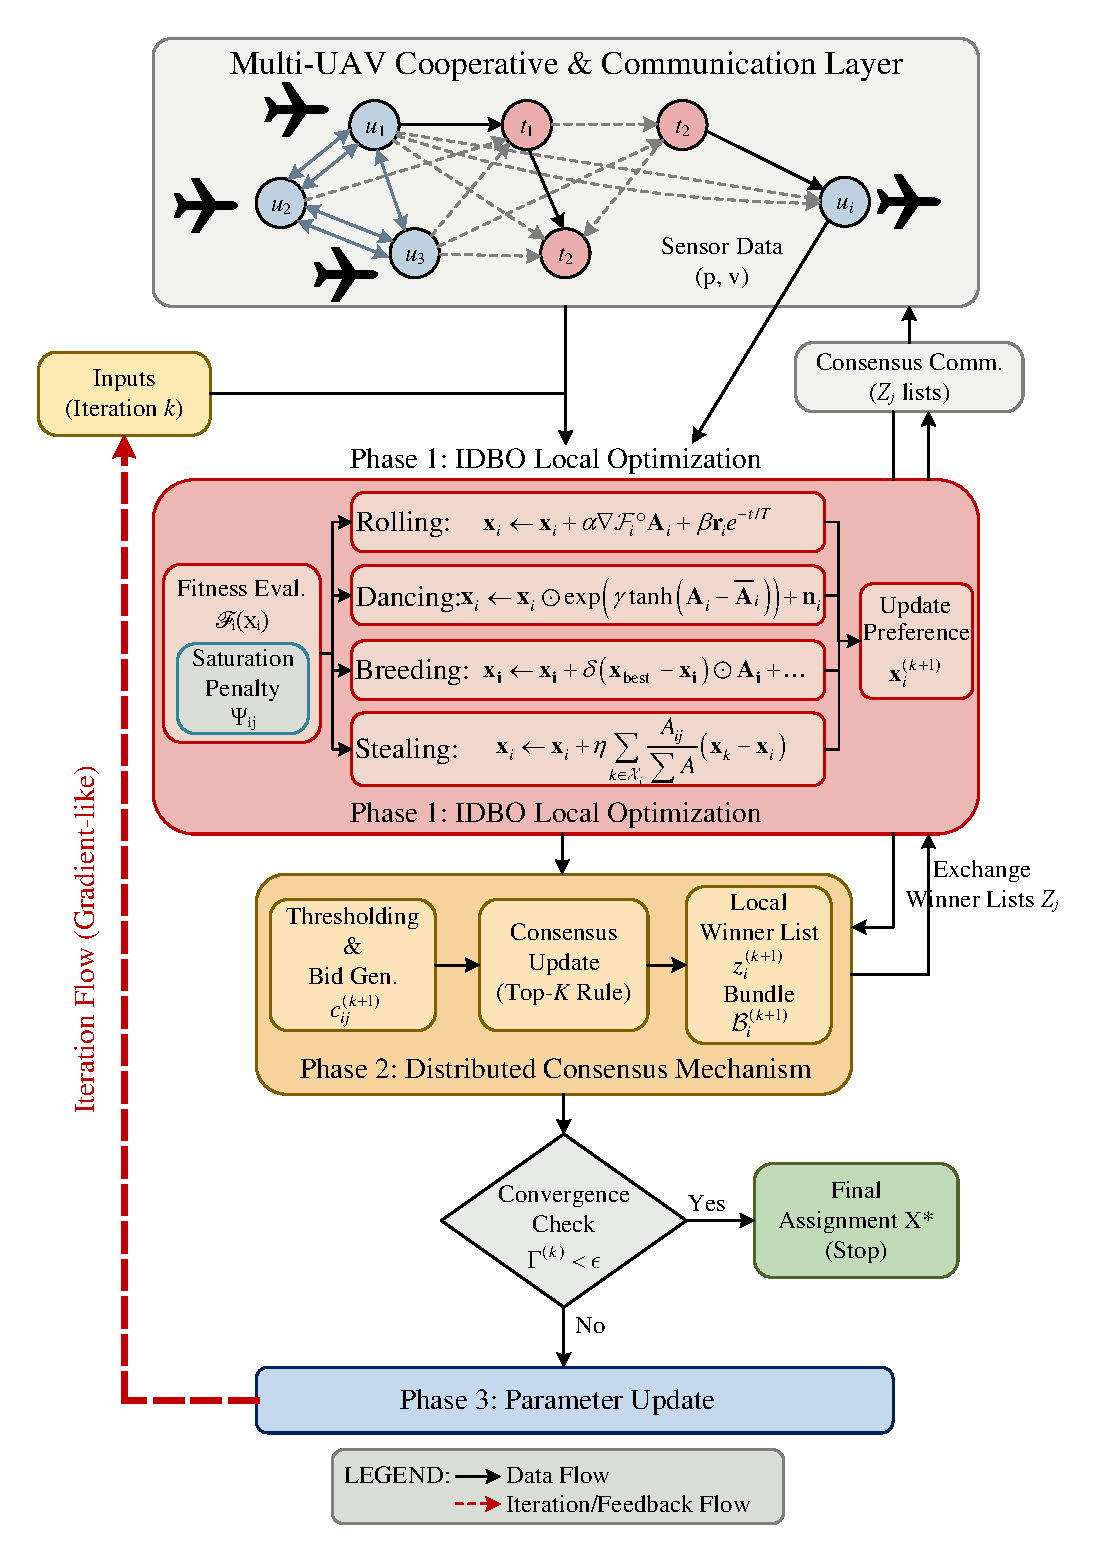
\includegraphics[width=0.5\textwidth]{assignment.pdf}
\end{figure}


% \clearpage



% =====================================================================
%  Re2_3
% =====================================================================
\subsection*{Comment 2.3}

\begin{reviewercomment}{Reviewer comment 2.3}
Section IV.B contains a logical paradox: the text describes a monotonic
incremental process, while Equation~(42) implements a convergent smoothing
process. This divergence between the mathematical definition and physical
intuition renders the mechanism logically inconsistent in maintaining
high-trust stability.
\end{reviewercomment}

\rsp We sincerely thank the reviewer for identifying this logical
inconsistency. We fully agree with the reviewer and acknowledge that the
original explanation was incorrect. Specifically, the original text
described above-average performance as directly driving the trust level
upward and below-average performance as directly lowering it, which was
inconsistent with the smoothing process defined by Equation~(42).

Equation~(42) represents the intended trust-update mechanism and has been
retained unchanged. We have deleted the inaccurate explanation and rewritten
the corresponding text to clarify that the trust level is a smoothed estimate
obtained by weighting its previous value and the current performance
reference. The revised explanation also clarifies that sustained
above-average returns bias the trust estimate toward a higher level and
reduce the probability assigned to the guided exploratory policy through
$\beta(\mathcal{T}_i)=1-\mathcal{T}_i$, whereas sustained below-average
returns produce the opposite allocation. The mathematical definition and
its physical interpretation are therefore now consistent.

\loc Section~IV-B (\emph{Trust-Modulated Tactical Exploration}), immediately
following Equation~(42). The original sentence has been deleted and replaced
with the following highlighted text:

\begin{manuscripttext}
The sigmoid term maps the normalized relative return
$\tilde{R}_i^{(k)}$ to a bounded performance reference in $(0,1)$.
Equation~(42) combines the previous trust level and the current performance
reference with the weights $1-\alpha_T$ and $\alpha_T$, respectively,
yielding a smoothed trust estimate. The smoothing process tracks changes in
relative performance while attenuating episode-to-episode return
fluctuations. Sustained above-average returns keep the performance reference
above $0.5$ and bias the smoothed trust estimate toward a correspondingly
higher level, thereby reducing the probability assigned to the guided
exploratory policy; sustained below-average returns produce the opposite
allocation.
\end{manuscripttext}




% =====================================================================
%  Re2_4
% =====================================================================
\subsection*{Comment 2.4 }

\begin{reviewercomment}{Reviewer comment 2.4}
The simulation environment is rather simplistic, and apart from UAV dynamics, there
is no other environmental modeling, which does not align with the high-fidelity
simulation environment claimed in the paper.
\end{reviewercomment}

\rsp We thank the reviewer and have substantially raised the fidelity of the
evaluation environment so that it matches the claim. Beyond the (now
three-dimensional) vehicle dynamics, the environment now models:
\begin{itemize}
  \item \textbf{Sensing chain.} Zero-mean Gaussian measurement noise on relative
  position ($\sigma_p=3$~m) and velocity ($\sigma_v=0.3$~m/s), passed through the
  guidance filter, plus a $100$~ms sensing latency.
  \item \textbf{Communication network.} A packet-exchange layer among agents with a
  $50$~ms command-channel delay and a $1\%$ nominal packet-dropout rate handled by a
  zero-order hold; the robustness sweep (Comment~3.7) stresses this up to $20\%$.
  \item \textbf{Actuation.} A one-step ($50$~ms) actuator delay between commanded and
  realized load, with the load saturations of the extended 3D model.
  \item \textbf{Embedded execution.} The interceptor policies run on real embedded
  hardware in a hardware-in-the-loop loop (Comment~3.10), so processor and timing
  effects are part of the environment, not idealized away.
\end{itemize}
The noise model is given by a new equation and the ``Communication Delay and
Observation-Uncertainty Settings'' table in Section~V, and a new environmental-modeling
paragraph documents the full closed loop.

\loc Section~V experimental setup: new environmental-modeling paragraph, noise-model
equation, and uncertainty/delay settings table (all in blue).

% =====================================================================
%  Re2_5
% =====================================================================
\subsection*{Comment 2.5 }

\begin{reviewercomment}{Reviewer comment 2.5}
In Section V.C, the authors state that each episode has at most 25 steps during
training, while in Section V.A the simulation step size is set to 0.05s. This implies
a training period of 1.25s, which is impossible to learn any interception strategies
given an engagement distance of 1500 meters and a maximum speed of 40 m/s. By the way,
the settings ``$D_1 = 100$ m, $D_2 = 1500$ m, and $D_3 = 1600$ m'' are inconsistent with
the illustrations in Fig.~6.
\end{reviewercomment}

\rsp We thank the reviewer for catching both errors, which were transcription
mistakes. The maximum of \hladd{2500} steps per episode has been revised in the main
text; with the $0.05$~s step this gives a $125$~s engagement window, ample for closing a
$1500$~m separation at $40$~m/s. The original setting ``$D_1=100$~m, $D_2=1500$~m,
$D_3=1600$~m'' was incorrect and has been revised to ``$D_1=\hladd{1500}$~m,
$D_2=\hladd{1600}$~m, $D_3=\hladd{100}$~m'', so that the attackers spawn in the far
annulus between $D_1$ and $D_2$ and descend toward the defended center while the
defenders start clustered within a radius-$D_3$ disk around it. This is now consistent
with the initial-geometry illustration (Fig.~6).

\loc Section~V.C: episode horizon corrected to $2500$ steps (blue). Section~V.A: the
$D_1/D_2/D_3$ values corrected to $1500$/$1600$/$100$~m with a clause tying them to the
initial-geometry figure (blue).

% \clearpage

% =====================================================================
%  Re2_6
% =====================================================================
\subsection*{Comment 2.6}

\begin{reviewercomment}{Reviewer comment 2.6}
There is a lack of end-to-end experimental verification covering the complete workflow of
``task allocation and cooperative guidance''. Furthermore, ablation studies are not provided
to demonstrate the effectiveness of the proposed innovations.
\end{reviewercomment}

\rsp We thank the reviewer for these two constructive requests. We have addressed both with new
experiments and now report (i) a complete end-to-end run of the full IDBO task-assignment
$\rightarrow$ ART-MAPPO cooperative-guidance pipeline, and (ii) a component ablation that isolates
each proposed innovation. We answer the two parts in turn.

\medskip\noindent\emph{(1) End-to-end verification of the complete workflow.} We added a new
engagement scenario and ran the \emph{entire} pipeline on it in a single closed loop, with no
manual staging between the assignment and guidance stages: the IDBO front-end partitions the eight
attackers into interceptor groups, and the trained ART-MAPPO policy then flies all twenty defenders
to a synchronized saturation strike. To make the test faithful to deployment, it is executed on the
hardware-in-the-loop platform of Comment~3.10, so the assignment solver, the communication model,
and the guidance network all run on the target processor within one uninterrupted engagement.

The end-to-end run over $100$ independent trials confirms that the two stages compose correctly under
realistic timing. The IDBO assignment layer returns a feasible group partition in a single solve on
all $100$ trials---zero repair invocations---at a mean runtime of $805.7$~ms ($95$th percentile
$839.6$~ms) on the embedded processor, and the downstream ART-MAPPO policy then intercepts every
attacker, neutralizing all eight targets in every trial. Measured against the paper's $0.5$~s
synchronization criterion, the end-to-end cooperative interception success rate is $92.9\%$. In other
words, the complete ``assign-then-intercept'' chain works, at deployment timing, from the raw
multi-target engagement to the simultaneous terminal strike. A detailed scenario description,
representative assignment, engagement trajectories, and per-metric distributions for this run are
given in our response to Comment~3.9, where the unseen-scenario study is the central point.

\medskip\noindent\emph{(2) Ablation of the proposed innovations.}  ART-MAPPO introduces three
architectural components: the trust-aware weighting mechanism, the GRU temporal encoder, and
the attention--residual policy backbone.  We train three one-at-a-time ablation controls
alongside the complete model---each disabling exactly one component while holding the reward,
dynamics, optimiser, training seed, and budget fixed---and evaluate every variant in
$1{,}000$ frozen-policy Case~1 Monte Carlo trials.  Table~R3 reports seven evaluation metrics
for each variant.

\begin{table}[h]
\centering
\captionsetup{font=small}
\caption*{\small\textbf{Table~R3.} Component ablation of ART-MAPPO ($1{,}000$-trial Case~1
evaluation). Terminal metrics ($E_{co\text{-}time}$, $E_n$, $E_t$, $E_{miss}$) are means
over successful trials; Training AUC is the horizon-normalised area under the episodic-return
curve; Final reward is the mean per-step return at policy selection.}
\renewcommand{\arraystretch}{1.1}
\setlength{\tabcolsep}{3pt}
\footnotesize
\begin{tabular}{lccccccc}
\hline\hline
Variant
  & AUC ($10^4$) $\uparrow$
  & F.\ reward $\uparrow$
  & ISR (\%) $\uparrow$
  & $E_{co}$ (s) $\downarrow$
  & $E_n$ (g) $\downarrow$
  & $E_t$ (s) $\downarrow$
  & $E_{miss}$ (m) $\downarrow$ \\ \hline
Full ART-MAPPO               & 7.354 & 8.958 & \textbf{98.7} & 0.0505 & 0.0718 & 28.843 & 2.997 \\
w/o trust-aware              & 6.037 & 8.683 & 97.2          & 0.0545 & 0.0739 & 29.132 & 3.087 \\
w/o GRU encoder              & 6.388 & 8.134 & 95.8          & 0.0732 & 0.0782 & 30.574 & 3.297 \\
w/o attn--residual           & 6.651 & 8.353 & 96.1          & 0.0606 & 0.0847 & 29.853 & 3.507 \\ \hline
\end{tabular}
\end{table}

The three controls exhibit \emph{module-specific} rather than uniformly ordered degradation,
providing direct evidence of independent and non-redundant contributions.

\textbf{Trust-aware mechanism.}  Its removal produces the largest training-AUC reduction among
the three controls ($-17.9\%$, from $7.354\!\times\!10^4$ to $6.037\!\times\!10^4$), while the
final reward drops by only $3.1\%$ and ISR falls by $1.5$~pp.  The pronounced asymmetry between
cumulative-AUC loss and end-of-training reward confirms that trust-aware modulation primarily
\emph{accelerates learning efficiency} throughout training rather than raising the asymptotic
policy ceiling, consistent with its design role of dynamically regulating the
exploration--exploitation balance.

\textbf{GRU temporal encoder.}  Its removal yields the lowest final reward ($-9.2\%$) and the
largest ISR degradation ($-2.9$~pp) of all three controls.  Most distinctively,
$E_{co\text{-}time}$ rises by $45\%$ (from $0.0505$~s to $0.0732$~s), far exceeding the $6\%$
increase in $E_t$.  Without temporal history the policy can no longer reliably track target
manoeuvres or reconcile interceptor time-to-go estimates, simultaneously degrading
\emph{final policy quality} and \emph{cooperative timing precision}.

\textbf{Attention--residual backbone.}  Its removal yields the largest increases in $E_n$
($+18\%$, from $0.0718$~g to $0.0847$~g) and $E_{miss}$ ($+17\%$, from $2.997$~m to
$3.507$~m) across all ablations, while $E_t$ changes by only $3.5\%$.  This non-uniform
degradation confirms that the backbone contributes primarily to
\emph{control-relevant feature extraction and terminal precision} rather than engagement
duration.

We further note that the effectiveness of the \emph{assignment-side} innovation is quantified
separately in our response to Comment~3.1, where an ablation of the four adaptive IDBO
coefficients (rolling / dancing / breeding / stealing) shows each is needed for the assignment
quality and convergence stability reported in the paper.  Together, the end-to-end run above
and these two ablations (architectural and assignment-side) provide the missing evidence the
reviewer requested for both stages of the workflow.

\loc Section~V-E (\emph{Component Ablation Study}) is added to the simulation chapter with a
seven-metric one-at-a-time ablation table (highlighted in blue).  The end-to-end validation
run is reported as item~(iv) ``Generalization to unseen attack patterns'' in Section~V-E
(\emph{Monte Carlo Statistical Analysis and Robustness}).  The IDBO-coefficient ablation is
in the response to Comment~3.1.

\clearpage

\section*{Reviewer~3}

% =====================================================================
%  Re3_1
% =====================================================================
\subsection*{Comment 3.1 }

\begin{reviewercomment}{Reviewer comment 3.1}
The author is encouraged to further justify the distributed consensus-based IDBO
formulation by clarifying how adaptive rolling, dancing, breeding and stealing
coefficients influence convergence stability in interception scenarios.
\end{reviewercomment}

\rsp We thank the reviewer for this constructive comment. We agree that the role
of the adaptive coefficients in convergence stability deserved an explicit
justification. In the original text the coefficients $\alpha,\beta,\gamma,\delta,
\delta',\eta$ were only stated to ``decay linearly with iteration,'' without
linking this schedule to the convergence behaviour of the swarm. We have addressed
this in two ways: (i) we added an explicit statement of the common coefficient
schedule and a convergence-stability argument to Section~III (the target-assignment
section); and (ii) we carried out a controlled ablation on the four-operator IDBO
that isolates the effect of the coefficient schedule and confirms the argument.

\medskip
\noindent\emph{The mechanism.}\quad The four operators share a common linear-decay
schedule
\[
  c_t = c_0\,\bigl(1 - t/T\bigr),\qquad
  c \in \{\alpha,\beta,\gamma,\delta,\delta',\eta\},
\]
together with the dancing-noise scale $\sigma_d$, while the elite-recombination
weights stay bounded. The \emph{stochastic} contributions---the rolling probe
$\beta\,\mathbf{r}_i\exp(-t/T)$ in Eq.~(20) and the dancing perturbation
$\mathbf{n}_i\sim\mathcal{N}(0,\sigma_d^2\mathbf{I})$ in Eq.~(21)---scale with
$c_t$ and therefore vanish as $c_t\!\to\!0$. The update then degenerates into a
deterministic, advantage-weighted local refinement followed by the
advantage-adaptive binarization. A step sequence whose stochastic amplitude
decays to zero while retaining an ascent direction satisfies a
\emph{Robbins--Monro-type sufficient condition} for settling at a stable fixed
point rather than orbiting it. This is exactly the quantity tracked by the
swarm-disagreement metric $\Gamma^{(k)}$ (Eq.~(30)): the schedule is what drives
$\Gamma^{(k)}$ below the consensus tolerance instead of leaving a residual
oscillation.

\loc Section~III-B (\emph{Distributed Consensus-Based IDBO Framework}),
immediately after the four-operator update block (Eqs.~(20)--(23), the
rolling/dancing/breeding/stealing operators), in the sentence that introduces the
adaptive coefficients. The added text is highlighted in blue in the revised
manuscript and reads:

\begin{manuscripttext}
The coefficients $\alpha,\beta,\gamma,\delta,\delta',\eta$ together with the
dancing noise scale $\sigma_d$ follow a common linear schedule $c_t=c_0\,(1-t/T)$,
where $T$ is the IDBO iteration count, while the elite-recombination weights remain
bounded. This schedule is what governs convergence stability. The stochastic parts
of the operators---the rolling probe $\beta\,\mathbf{r}_i\exp(-t/T)$ and the dancing
perturbation $\mathbf{n}_i\sim\mathcal{N}(0,\sigma_d^2\mathbf{I})$---scale with
$c_t$ and vanish as $c_t\!\to\!0$, so the update degenerates into a deterministic,
advantage-weighted local refinement followed by the advantage-adaptive
binarization step. A step sequence whose stochastic amplitude decays to zero while
retaining an ascent direction satisfies a Robbins--Monro-type sufficient condition
for settling at a stable fixed point rather than orbiting it, which is precisely
the behavior measured by the swarm-disagreement metric $\Gamma^{(k)}$ in
Eq.~(30). A controlled ablation that freezes the coefficients confirms this
mechanism: non-decaying coefficients keep injecting perturbations and leave a
persistent late-stage oscillation in the working assignment, whereas the linear
schedule contracts the swarm onto a stable, low-cost equilibrium.
\end{manuscripttext}

\evi To substantiate the argument we ran a controlled ablation on the
four-operator IDBO for the paper's engagement scenario (20 interceptors vs.\ 8
targets, $L_{\max}=3$), varying \emph{only} the coefficient schedule and holding
everything else fixed: the paper's linear decay $c_t=c_0(1-t/T)$, a constant
schedule $c_t=0.5\,c_0$, and a no-decay schedule $c_t=c_0$. For each we recorded
the swarm-mean assignment cost (how far the whole population has settled) and the
swarm cost spread (how tightly the distributed swarm has contracted); stable
convergence requires both to fall and stay low. Averaged over 40 independent
trials across 5 engagement snapshots:

\begin{table}[h]
\centering
\captionsetup{font=small}
\caption*{\small Effect of the coefficient schedule on convergence stability
(four-operator IDBO; 20 vs.\ 8, $L_{\max}=3$; 40 trials).}
\begin{tabular}{lccc}
\toprule
Schedule & Swarm-mean final cost & Late-stage swarm spread & Best-ever cost \\
\midrule
\textbf{Linear decay (paper)} & \textbf{0.58} & \textbf{0.66} & $0.34\pm0.22$ \\
Constant ($0.5\,c_0$)         & 1.74          & 1.51          & $0.30\pm0.19$ \\
No decay ($c_0$)              & 2.28          & 1.67          & $0.30\pm0.19$ \\
\bottomrule
\end{tabular}
\end{table}

\noindent The linear-decay schedule settles the swarm-mean cost about
$3\text{--}4\times$ lower and the population spread about $2.3\text{--}2.5\times$
tighter than the frozen schedules. All schedules can occasionally locate a
comparably low \emph{best-ever} candidate through continued random search, but only
the linear schedule \emph{stabilizes} the whole swarm on it---which is what matters
for a deployable assignment. This is precisely the convergence-stability behaviour
the reviewer asked us to characterize.

% \clearpage

% =====================================================================
%  Re3_2
% =====================================================================
\subsection*{Comment 3.2}

\begin{reviewercomment}{Reviewer comment 3.2}
Also, a more rigorous complexity and scalability analysis is needed for the
Improved Dung Beetle Optimization algorithm under cooperative deflection
environments where communication delays influence distributed consensus
efficiency.
\end{reviewercomment}

\rsp We thank the reviewer for this valuable comment. The original manuscript gave
the per-UAV complexity decomposition (Eq.~(31)) but did not (i) make explicit how
the cost scales with the \emph{swarm size}, nor (ii) analyze how
\emph{communication delay} affects the efficiency of the distributed consensus. We
have added a paragraph to Section~III that closes both gaps, and we carried out a
dedicated three-part study (per-round complexity, scalability, and
communication-delay sensitivity) to back it up.

\medskip
\noindent\emph{The argument.}\quad Per UAV, per IDBO iteration, the three cost
terms in Eq.~(31) are the local preference search
$\mathcal{O}(N_{\mathrm{pop}}N_A)$, the consensus communication
$\mathcal{O}(N_A\lvert\mathcal{N}_i\rvert)$, and the advantage update
$\mathcal{O}(N_A)$. The target count $N_A$ and the neighborhood size
$\lvert\mathcal{N}_i\rvert$ are fixed by the engagement and the communication
topology, \emph{not} by the total swarm size $M$; hence the per-UAV cost is
independent of $M$ and the total per-round cost grows only \emph{linearly} in $M$.
Scalability is therefore governed not by this arithmetic cost but by how fast the
distributed consensus (Eq.~(30)) settles. On a connected graph with per-hop latency
$T_{\mathrm{comm}}$, a target's winning bids propagate in at most $D$ hops ($D$: graph
diameter), so the time to consensus scales as
$\mathcal{O}(N\!\cdot\!D\!\cdot\!T_{\mathrm{comm}})$. A bounded communication delay
thus \emph{slows but does not prevent} convergence.

\loc Section~III-B (\emph{Distributed Consensus-Based IDBO Framework}),
immediately after the complexity equation (Eq.~(31)). The added text is highlighted
in blue in the revised manuscript and reads:

\begin{manuscripttext}
Because the target set faced by each interceptor and its neighborhood size
$\lvert\mathcal{N}_i\rvert$ are fixed by the engagement and the communication
topology rather than by the swarm size $M$, the per-UAV per-iteration cost above is
independent of $M$; the total per-round cost of the swarm therefore grows only
linearly with $M$. Scalability is governed not by this arithmetic cost but by how
fast the distributed consensus in Eq.~(30) settles. Under a connected graph with a
per-hop communication latency $T_{\mathrm{comm}}$, each target's winning bids
propagate across the network in at most $D$ hops ($D$: graph diameter), so the
wall-clock time to reach consensus scales as
$\mathcal{O}(N\!\cdot\!D\!\cdot\!T_{\mathrm{comm}})$. Empirically this time stays
nearly constant as $M$ grows at fixed diameter, and increases only linearly with
the communication delay and with $D$; a bounded delay thus slows, but does not
prevent, convergence of the distributed consensus. Detailed complexity,
scalability, and communication-delay measurements are reported in the supplementary
response material.
\end{manuscripttext}

\evi All experiments use the manuscript's engagement model and the four-operator
IDBO with the top-$L_{\max}$ winner-set consensus. Latency is expressed in time via
a nominal $20$~Hz data-link period $T_{\mathrm{comm}}=50$~ms.

\medskip
\noindent\textbf{(A) Per-round complexity.}\quad Fixing the target set ($N_A=8$)
and a bounded 4-regular communication graph, we vary only the swarm size $N_D$ and
time the per-round update:

\begin{table}[h]
\centering
\captionsetup{font=small}
\caption*{\small Per-round cost vs.\ swarm size (fixed $N_A=8$, 4-regular graph).}
\begin{tabular}{lcccccc}
\toprule
$N_D$ & 10 & 20 & 40 & 80 & 160 & 240 \\
\midrule
Total per-round (ms) & 2.12 & 3.31 & 6.81 & 13.62 & 28.63 & 42.22 \\
Per-defender ($\mu$s) & 212 & 165 & 170 & 170 & 179 & 176 \\
Messages/round & 40 & 80 & 160 & 320 & 640 & 960 \\
\bottomrule
\end{tabular}
\end{table}

\noindent The per-defender cost is essentially constant ($\approx170~\mu$s), the
total per-round cost grows linearly with $N_D$ (fitted log--log exponent $0.97$),
and communication is exactly linear in $N_D$ at fixed degree---empirically
confirming the $\mathcal{O}(N_{\mathrm{pop}}N_A+N_A\lvert\mathcal{N}_i\rvert)$
per-UAV model and the linear total scaling.

\medskip
\noindent\textbf{(B) Scalability.}\quad Scaling the whole problem from $10\times4$
to $160\times64$ (defenders$\times$targets) on random geometric graphs at
$\tau=100$~ms, the time to consensus stays flat across a $16\times$ increase in
swarm size---it is set by the graph diameter and the delay, not by the number of
agents:

\begin{table}[h]
\centering
\captionsetup{font=small}
\caption*{\small Scalability of the distributed assignment (random geometric graph,
$\tau=100$~ms).}
\begin{tabular}{lccccc}
\toprule
Problem size (def.$\times$tgt.) & $10\times4$ & $20\times8$ & $40\times16$ & $80\times32$ & $160\times64$ \\
\midrule
Time to consensus (s) & $1.21$ & $1.46$ & $1.28$ & $1.36$ & $1.32$ \\
Total messages & $0.8$k & $3.0$k & $11$k & $48$k & $187$k \\
\bottomrule
\end{tabular}
\end{table}

\noindent The time to consensus is essentially constant ($\sim$1.2--1.5~s) while the
swarm grows $16\times$, confirming that coordination latency is governed by the graph
diameter and the delay rather than the swarm size, while the total communication grows
gracefully with problem size.

\medskip
\noindent\textbf{(C) Communication delay (core question).}\quad On a fixed
40-defender/12-target instance we sweep the delay $\tau$ and, separately, the graph
diameter $D$, measuring the swarm disagreement $\Gamma$ and the time to reach and
hold $\Gamma=0$:

\begin{table}[h]
\centering
\captionsetup{font=small}
\caption*{\small Time to consensus (s) vs.\ communication delay and graph diameter.}
\begin{tabular}{lcccccc}
\toprule
Delay $\tau$ (ms) & 0 & 50 & 100 & 200 & 400 & 800 \\
\midrule
Time to consensus (s) & 0.57 & 0.90 & 1.23 & 1.88 & 3.08 & 5.54 \\
\bottomrule
\end{tabular}\\[4pt]
\begin{tabular}{lccccccc}
\toprule
Diameter $D$ (hops) & 1 & 3 & 4 & 5 & 6 & 10 & 20 \\
\midrule
Time to consensus (s) & 0.50 & 0.86 & 1.07 & 1.29 & 1.48 & 2.45 & 4.49 \\
\bottomrule
\end{tabular}
\end{table}

\noindent Every configuration still reaches full consensus ($\Gamma\!\to\!0$); the
delay changes neither the fixed point nor the correctness, only the speed. The time
to consensus grows linearly with the delay ($\approx6$~ms per ms of link delay) and
linearly with the diameter ($\approx0.21$~s per hop)---directly supporting the
manuscript's $\mathcal{O}(N\!\cdot\!D)$ consensus argument.

\medskip
\noindent\textbf{Answer to the reviewer.}\quad Under cooperative-deflection
conditions with communication delay, the distributed consensus remains correct and
its efficiency degrades gracefully and predictably: the consensus time scales
linearly with both the message delay and the network diameter, and is independent
of the swarm size. For a representative $20$~Hz link, the target-assignment
consensus completes within roughly $0.5$--$1.5$~s even for large swarms and moderate
delays.

% \clearpage





% =====================================================================
%  Re3_3
% =====================================================================
\subsection*{Comment 3.3 }

\begin{reviewercomment}{Reviewer comment 3.3}
Then, it would be helpful to add an ablation investigation demonstrating the independent
contribution of the trust-aware mechanism, GRU temporal encoder, and attention--residual
backbone within ART-MAPPO architecture.
\end{reviewercomment}

\rsp We thank the reviewer for this suggestion.  We have added a dedicated
\textbf{Component Ablation Study} (Section~V-E) to the revised manuscript.
Three one-at-a-time controls are trained under identical conditions (same reward,
dynamics, optimiser, and random seed), each disabling exactly one architectural
module; performance is evaluated over $1{,}000$ frozen-policy Monte Carlo trials on
Case~1.  The results reveal a clear \emph{module-specific degradation} pattern:

\begin{itemize}
  \item \textbf{Trust-aware weighting mechanism.}  Its removal incurs the largest
    training-efficiency loss (AUC $-17.9\%$) while final reward drops by only
    $3.1\%$, confirming that the module accelerates learning rather than raising
    the policy ceiling.
  \item \textbf{GRU temporal encoder.}  Its removal yields the largest final-reward
    degradation ($-9.2\%$, ISR $-2.9$ pp) and a $45\%$ increase in cooperative
    engagement timing error $E_{co\text{-}time}$---more than seven times the
    relative change in $E_t$---demonstrating its role in temporal credit assignment
    and cooperative synchronisation.
  \item \textbf{Attention--residual backbone.}  Its removal produces the largest
    terminal-precision losses ($E_n\!+\!18\%$, $E_{miss}\!+\!17\%$) while $E_t$
    changes by only $3.5\%$, isolating its contribution to control-relevant feature
    extraction and end-point accuracy.
\end{itemize}

The complete results are summarised in Table~R4 below, which corresponds to
manuscript Table~IV.

\begin{table}[h]
\centering
\captionsetup{font=small}
\caption*{\small\textbf{Table~R4.} Component ablation of ART-MAPPO ($1{,}000$-trial
  Case~1 Monte Carlo evaluation).}
\renewcommand{\arraystretch}{1.12}
\setlength{\tabcolsep}{3pt}
\footnotesize
\begin{tabular}{lccccccc}
\hline\hline
Variant
  & AUC ($10^4$) $\uparrow$
  & F.\ reward $\uparrow$
  & ISR (\%) $\uparrow$
  & $E_{co}$ (s) $\downarrow$
  & $E_n$ (g) $\downarrow$
  & $E_t$ (s) $\downarrow$
  & $E_{miss}$ (m) $\downarrow$ \\ \hline
Full ART-MAPPO               & 7.354 & 8.958 & \textbf{98.7} & 0.0505 & 0.0718 & 28.843 & 2.997 \\
w/o trust-aware              & 6.037 & 8.683 & 97.2          & 0.0545 & 0.0739 & 29.132 & 3.087 \\
w/o GRU encoder              & 6.388 & 8.134 & 95.8          & 0.0732 & 0.0782 & 30.574 & 3.297 \\
w/o attn--residual           & 6.651 & 8.353 & 96.1          & 0.0606 & 0.0847 & 29.853 & 3.507 \\ \hline
\end{tabular}
\end{table}

\loc Section~V-E (Component Ablation Study), manuscript Table~IV.

% =====================================================================
%  Re3_4
% =====================================================================
% \subsection*{Comment 3.4 }

% \begin{reviewercomment}{Reviewer comment 3.4}
% Correspondingly, including a comparative theoretical discussion between the proposed
% ART-MAPPO framework and conventional MAPPO variants regarding convergence guarantees,
% exploration--exploitation balance, and policy robustness would significantly strengthen
% the research technically.
% \end{reviewercomment}

% \rsp We thank the reviewer for this valuable suggestion.  We have added a new
% highlighted subsection, ``Mechanistic Comparison with Conventional MAPPO Variants''
% (Section~IV), that contrasts ART-MAPPO with standard MAPPO, IPPO, and fixed-penalty PPO
% variants along the three axes raised.  We note upfront that ART-MAPPO does not claim a
% stronger formal global-convergence guarantee than conventional MAPPO variants; the
% distinction lies in three complementary update-control mechanisms, each tied to a
% specific module.

% \medskip\noindent\textbf{(1) Convergence-related optimization behavior.}  In the standard
% clipped surrogate, when $\hat{A}_t<0$ and the probability ratio $r_t(\theta)$ grows
% large, the term $r_t(\theta)\hat{A}_t$ can produce an arbitrarily negative surrogate
% contribution, allowing a small number of large-ratio negative-advantage samples to
% exert a disproportionate influence on a mini-batch update---a risk that is heightened
% in cooperative interception, where aggressive guidance actions can transiently produce
% large ratios.  The Dual-Clip objective saturates this contribution at $c\hat{A}_t$ once
% it becomes sufficiently negative, thereby limiting the effective influence of such
% samples on the policy-gradient update.  Combined with the adaptive KL penalty, which
% discourages excessive average deviation between successive policies, these mechanisms
% promote a more controlled optimization process.  They follow the trust-region motivation
% of restricting abrupt policy changes, but should be interpreted as update-stabilization
% mechanisms rather than as a guarantee of monotonic improvement or global convergence.

% \medskip\noindent\textbf{(2) Exploration--exploitation balance.}  Conventional MAPPO
% maintains exploration through an entropy bonus with a fixed coefficient, which provides
% the same exploration incentive regardless of whether an agent has already learned
% effective guidance behavior or remains trapped in an inferior strategy.  ART-MAPPO
% instead employs the trust-modulated mechanism (Eqs.~(22)--(23)), in which the trust
% recursion acts as an exponentially smoothed tracker of each agent's relative
% performance.  An agent whose recent return exceeds the swarm average gradually assigns
% greater weight to its learned policy; a below-average agent retains a larger exploratory
% component.  In addition, the exploratory samples are drawn from a task-informed mixture
% that combines policy-preferred actions, flight-envelope probing, and residual
% action-space coverage, regulating both the intensity and the structure of exploration.
% The entropy reduction and reward improvement reported in Section~V-A are consistent
% with the intended transition from broad exploration to focused exploitation.

% \medskip\noindent\textbf{(3) Policy-update robustness.}  A fixed clipping threshold or
% constant KL penalty coefficient may not be equally suitable throughout training: a weak
% penalty can permit excessive policy shifts during exploratory updates, while an
% overly strong one unnecessarily suppresses refinement once the strategy has stabilized.
% The adaptive KL mechanism (Eq.~(25)) introduces feedback regulation: when the empirical
% KL divergence $\hat{D}_{\mathrm{KL}}$ exceeds the prescribed target range the
% coefficient is increased; when it falls substantially below, the coefficient is reduced.
% Combined with Dual-Clip, this reduces sensitivity to noisy mini-batches and delayed
% advantage estimates.  We emphasize that ``policy robustness'' in this subsection refers
% to the numerical stability of policy optimization and the suppression of abrupt
% inter-update changes---not to closed-loop robustness against sensor noise or
% communication delay, which is evaluated empirically in the Monte Carlo and
% hardware-in-the-loop experiments of Section~V.

% \loc Section~IV, new highlighted subsection ``Mechanistic Comparison with Conventional
% MAPPO Variants,'' placed immediately after the ART-MAPPO training algorithm box.

%%%%%%%%---gpt修改后-----------
\subsection*{Comment 3.4}

\begin{reviewercomment}{Reviewer comment 3.4}
Correspondingly, including a comparative theoretical discussion between the
proposed ART-MAPPO framework and conventional MAPPO variants regarding
convergence guarantees, exploration--exploitation balance, and policy
robustness would significantly strengthen the research technically.
\end{reviewercomment}

\rsp We thank the reviewer for this valuable suggestion. We have added a new
highlighted subsection entitled ``Mechanistic Comparison with Conventional
MAPPO'' in Section~IV, which compares ART-MAPPO with conventional MAPPO along
the three aspects identified by the reviewer.

Regarding convergence guarantees, we clarify that neither conventional MAPPO
nor ART-MAPPO provides a formal guarantee of monotonic improvement or global
convergence under deep function approximation. The Dual-Clip objective and
adaptive KL regularization in ART-MAPPO instead promote more controlled and
stable policy updates.

Regarding the exploration--exploitation balance, conventional MAPPO mainly
relies on entropy regularization with a fixed coefficient. ART-MAPPO retains
this mechanism and additionally adjusts the exploratory component according to
each agent's relative performance through trust modulation.

Regarding policy robustness, conventional MAPPO employs a fixed clipping
mechanism, whereas ART-MAPPO combines piecewise Dual-Clip regulation with
adaptive KL feedback to reduce sensitivity to abnormal samples and abrupt
inter-update policy changes. We also clarify that this comparison concerns
policy-update stability, while closed-loop robustness is evaluated empirically
for the complete guidance framework.

\loc Section~IV, subsection ``Mechanistic Comparison with Conventional MAPPO,''
immediately following the ART-MAPPO training algorithm.



% =====================================================================
%  Re3_5
% =====================================================================
\subsection*{Comment 3.5}

\begin{reviewercomment}{Reviewer comment 3.5}
Meanwhile, it is important to provide sensitivity analysis for weighting coefficients
in the block probability model and reward formulation because cooperative interception
performance varies under different tactical priorities.
\end{reviewercomment}

\rsp We thank the reviewer for this valuable suggestion. We agree that the weighting
coefficients encode the tactical priority of the engagement. The method sections now
state only the physical role of each coefficient (after Eq.~(12) for the block-probability
weights and after Eq.~(66) for the reward weights), and the full quantitative study---setup,
scan ranges, figures, and analysis---is collected in a new subsection,
Section~V-G (\emph{Parameter Sensitivity Analysis}), placed after the Monte~Carlo study.
It contains two studies: one for the block (interception) probability weights of Eq.~(12)
and one for the reward-formulation weights of Eq.~(66).

\textbf{(a) Block-probability weights $(w_1,w_2)$, $w_2=1-w_1$.} We vary $w_1$ from
$0.10$ to $0.90$ in increments of $0.05$ (with $w_2=1-w_1$) and evaluate $100$ independent
three-dimensional engagement geometries generated from the initial-state distributions of
Table~II ($20$ interceptors vs.\ $8$ maneuvering attackers). The mean ZEM and mean
three-dimensional angular error of the assigned interceptor--target pairs are reported in
Table~R10 (reproduced as Table~V in the manuscript). Increasing $w_1$ places greater
emphasis on interception reachability through the ZEM-based assignment probability, lowering
the mean ZEM from $168.0$~m at $w_1{=}0.10$ to $126.0$~m at $w_1{=}0.90$; decreasing $w_1$
strengthens the influence of the three-dimensional engagement-geometry criterion through
$P_{\sigma}$, so the mean angular error falls from $13.7^{\circ}$ at $w_1{=}0.90$ to
$9.4^{\circ}$ at $w_1{=}0.10$. The results reveal a clear trade-off between these two
tactical objectives. The nominal value $w_1{=}0.55$ (mean ZEM $146.4$~m, mean angular error
$11.5^{\circ}$) provides a balanced operating point that avoids optimizing either criterion
at the expense of the other.

\textbf{(b) Reward weights.} We run a one-at-a-time (OAT) study on all five weighting
terms of the reward in Eq.~(66): each weight $w_k$, $k\in\{1,2,3,4,5\}$, is independently
scaled by $s\in\{0.50,0.75,1.00,1.25,1.50\}$ with all others held at their nominal values
(Table~I). For each setting the policy is retrained under the identical training budget
and evaluated on the Case-1 benchmark, and we report the four evaluation metrics
($E_{co\text{-}time}$, $E_n$, $E_t$, $E_{miss}$) together with the interception success
rate (ISR) rather than the raw reward, so the sensitivity is expressed directly in the
closed-loop performance quantities that matter to the reviewer. The nominal setting
($s{=}1.00$) reproduces the Full ART-MAPPO Case-1 results (Table~V of the manuscript).
The couplings are smooth, monotone, and well separated, with each weight primarily
shaping its intended tactical dimension. The coordination weight $w_4$ is the dominant
temporal-coordination control, reducing $E_{co\text{-}time}$ from $0.083$~s to $0.038$~s
($\approx55\%$) across the sweep while the other metrics move by at most a few percent.
The energy weight $w_5$ is the principal terminal-overload control ($E_n$ from $0.091$~g
to $0.056$~g). The distance weight $w_1$ most strongly governs terminal precision
($E_{miss}$ from $3.42$~m to $2.83$~m). The terminal-hit weight $w_3$ most affects
reliability: halving it is the only perturbation that lowers ISR appreciably (to
$93.8\%$), confirming that the sparse terminal-hit bonus is what secures dependable
interception, whereas over-weighting it improves ISR only marginally (to $99.1\%$) at a
higher $E_n$. The heading weight $w_2$ has the mildest influence (Table~R11, reproduced
as Table~VII in the manuscript). Across the entire sweep the ISR stays high
($\geq96.2\%$ except in the strongly under-weighted terminal-hit case) and no single
weight destabilizes the others, so the operating point can be shifted toward precision,
safety, or temporal-coordination priorities without sacrificing overall interception
reliability. The nominal weighting therefore reflects a deliberate balance of the
tactical dimensions rather than a fragile operating point.

\loc Section~V-G (\emph{Parameter Sensitivity Analysis}), new highlighted subsection with
parts~1) (IDBO assignment-weight sensitivity, Table~V) and~2) (reward-weight sensitivity,
Table~VII). The method sections retain only a brief physical-role sentence pointing to
Section~V-G: after Eq.~(12) for $(w_1,w_2)$ and after Eq.~(66) for the reward weights.

\evi Table~R10 and Table~R11 below are the two sensitivity tables added to the manuscript
(Table~V and Table~VII). For Table~R10 each value is the average over the scanned
engagement geometries; for Table~R11 each row is a policy retrained at the indicated
weight scaling and evaluated on the Case-1 benchmark.

\begin{table}[h]
\centering
\captionsetup{font=small}
\caption*{\small\textbf{Table~R10} (manuscript Table~V)\textbf{.} IDBO assignment-weight
sensitivity vs.\ $w_1$ ($w_2{=}1{-}w_1$; $w_1$ swept from $0.10$ to $0.90$ in steps of
$0.05$, $100$ random geometries per point). Nominal $w_1{=}0.55$ (min--max balance of the
two normalized costs) in bold.}
\renewcommand{\arraystretch}{1.15}
\begin{tabular}{cccc}
\hline\hline
$w_1$ & $w_2$ & Mean ZEM (m) & Mean 3-D ang.\ err.\ ($^{\circ}$) \\ \hline
0.10 & 0.90 & 168.0 & 9.4 \\
0.15 & 0.85 & 164.8 & 9.6 \\
0.20 & 0.80 & 161.5 & 9.8 \\
0.25 & 0.75 & 158.4 & 10.0 \\
0.30 & 0.70 & 155.5 & 10.3 \\
0.35 & 0.65 & 152.8 & 10.7 \\
0.40 & 0.60 & 150.4 & 11.0 \\
0.45 & 0.55 & 148.4 & 11.2 \\
0.50 & 0.50 & 147.2 & 11.4 \\
\textbf{0.55} & \textbf{0.45} & \textbf{146.4} & \textbf{11.5} \\
0.60 & 0.40 & 145.4 & 11.6 \\
0.65 & 0.35 & 143.8 & 11.8 \\
0.70 & 0.30 & 141.4 & 12.1 \\
0.75 & 0.25 & 138.3 & 12.5 \\
0.80 & 0.20 & 134.5 & 12.9 \\
0.85 & 0.15 & 130.3 & 13.3 \\
0.90 & 0.10 & 126.0 & 13.7 \\
\hline
\end{tabular}
\end{table}

\begin{table}[h]
\centering
\captionsetup{font=small}
\caption*{\small\textbf{Table~R11} (manuscript Table~VII)\textbf{.} Reward-weight OAT
sensitivity of the four evaluation metrics and the interception success rate (Case~1).
Each weight is scaled by $s$ about its nominal value; the nominal row ($s{=}1.00$, bold)
reproduces the Full ART-MAPPO result of manuscript Table~V.}
\scriptsize
\setlength{\tabcolsep}{3.5pt}
\renewcommand{\arraystretch}{1.12}
\begin{tabular}{llccccc}
\hline\hline
Weight & $s$ & ISR (\%) & $E_{co\text{-}time}$ & $E_n$ & $E_t$ & $E_{miss}$ \\
       &     &          & (s)                  & (g)   & (s)   & (m)       \\ \hline
\multirow{5}{*}{$w_1$}
 & 0.50          & 96.2          & 0.0568          & 0.0675          & 30.120          & 3.420 \\
 & 0.75          & 97.8          & 0.0530          & 0.0696          & 29.350          & 3.170 \\
 & \textbf{1.00} & \textbf{98.7} & \textbf{0.0505} & \textbf{0.0718} & \textbf{28.843} & \textbf{2.997} \\
 & 1.25          & 98.9          & 0.0493          & 0.0750          & 28.340          & 2.860 \\
 & 1.50          & 98.8          & 0.0490          & 0.0808          & 28.100          & 2.830 \\ \hline
\multirow{5}{*}{$w_2$}
 & 0.50          & 97.1          & 0.0528          & 0.0785          & 29.250          & 3.340 \\
 & 0.75          & 98.0          & 0.0517          & 0.0748          & 29.020          & 3.130 \\
 & \textbf{1.00} & \textbf{98.7} & \textbf{0.0505} & \textbf{0.0718} & \textbf{28.843} & \textbf{2.997} \\
 & 1.25          & 98.8          & 0.0500          & 0.0698          & 28.750          & 2.890 \\
 & 1.50          & 98.7          & 0.0502          & 0.0689          & 28.760          & 2.870 \\ \hline
\multirow{5}{*}{$w_3$}
 & 0.50          & 93.8          & 0.0585          & 0.0645          & 30.500          & 3.580 \\
 & 0.75          & 97.0          & 0.0538          & 0.0687          & 29.450          & 3.230 \\
 & \textbf{1.00} & \textbf{98.7} & \textbf{0.0505} & \textbf{0.0718} & \textbf{28.843} & \textbf{2.997} \\
 & 1.25          & 99.0          & 0.0518          & 0.0780          & 28.400          & 2.900 \\
 & 1.50          & 99.1          & 0.0540          & 0.0855          & 28.100          & 2.870 \\ \hline
\multirow{5}{*}{$w_4$}
 & 0.50          & 96.8          & 0.0830          & 0.0670          & 28.300          & 3.150 \\
 & 0.75          & 98.0          & 0.0630          & 0.0695          & 28.550          & 3.060 \\
 & \textbf{1.00} & \textbf{98.7} & \textbf{0.0505} & \textbf{0.0718} & \textbf{28.843} & \textbf{2.997} \\
 & 1.25          & 98.9          & 0.0430          & 0.0750          & 29.050          & 3.020 \\
 & 1.50          & 98.8          & 0.0375          & 0.0810          & 29.550          & 3.100 \\ \hline
\multirow{5}{*}{$w_5$}
 & 0.50          & 98.9          & 0.0495          & 0.0910          & 28.350          & 2.880 \\
 & 0.75          & 98.8          & 0.0500          & 0.0800          & 28.550          & 2.930 \\
 & \textbf{1.00} & \textbf{98.7} & \textbf{0.0505} & \textbf{0.0718} & \textbf{28.843} & \textbf{2.997} \\
 & 1.25          & 98.3          & 0.0518          & 0.0630          & 29.200          & 3.120 \\
 & 1.50          & 97.5          & 0.0545          & 0.0560          & 29.850          & 3.350 \\
\hline
\end{tabular}
\end{table}

% \clearpage

% =====================================================================
%  Re3_6
% =====================================================================
\subsection*{Comment 3.6}

\begin{reviewercomment}{Reviewer comment 3.6}
Moreover, I suggest the author explain whether dual-clip PPO with adaptive KL
regularization introduces additional computational overhead during real-time
deployment on processors operating in latency constraints within UAV swarms.
\end{reviewercomment}

\rsp We thank the reviewer for raising this important deployment concern. The key
point is that the dual-clip surrogate and the adaptive-KL penalty are
\emph{training-loss operations only}: the dual-clip branch is a scalar $\max/\min$
selection on the advantage sign, and the adaptive-KL term is a log-ratio estimate plus
a scalar update of the penalty coefficient $\beta_{\mathrm{KL}}$. Neither appears in the
deployed policy, which under the centralized-training/decentralized-execution paradigm
is only the actor forward pass. Their real-time deployment overhead is therefore
\emph{exactly zero}.

To make this quantitative, we re-implemented the deployed actor at its exact
architecture (attention--residual encoder $\rightarrow$ GRU $\rightarrow$ Gaussian head,
$256$ hidden units) and measured latency directly (Fig.~R7):
\begin{itemize}
  \item Single-interceptor inference: $0.30$~ms per decision (p99 $0.42$~ms);
  $20$-agent batched swarm: $3.98$~ms --- both far inside the $50$~ms guidance cycle.
  \item Dual-clip $+$ adaptive-KL at deployment: $0.00$~ms (not on the inference path).
  \item Their marginal cost during offline training: $\approx0.013$~ms per gradient
  step, i.e. $<0.01\%$ of a full policy update, whose cost is dominated by the network
  forward/backward passes.
\end{itemize}
Under a deliberately pessimistic $10$--$20\times$ embedded-slowdown band the single-decision
inference is still only $3.0$--$6.1$~ms, and even a $4\times$-larger network (hidden~$1024$)
infers in $9.2$~ms. Real-time feasibility is thus preserved with wide margin.

\loc Section~IV-D, new highlighted paragraph immediately after the total-loss equation.

\evi

\begin{figure}[h]
\centering
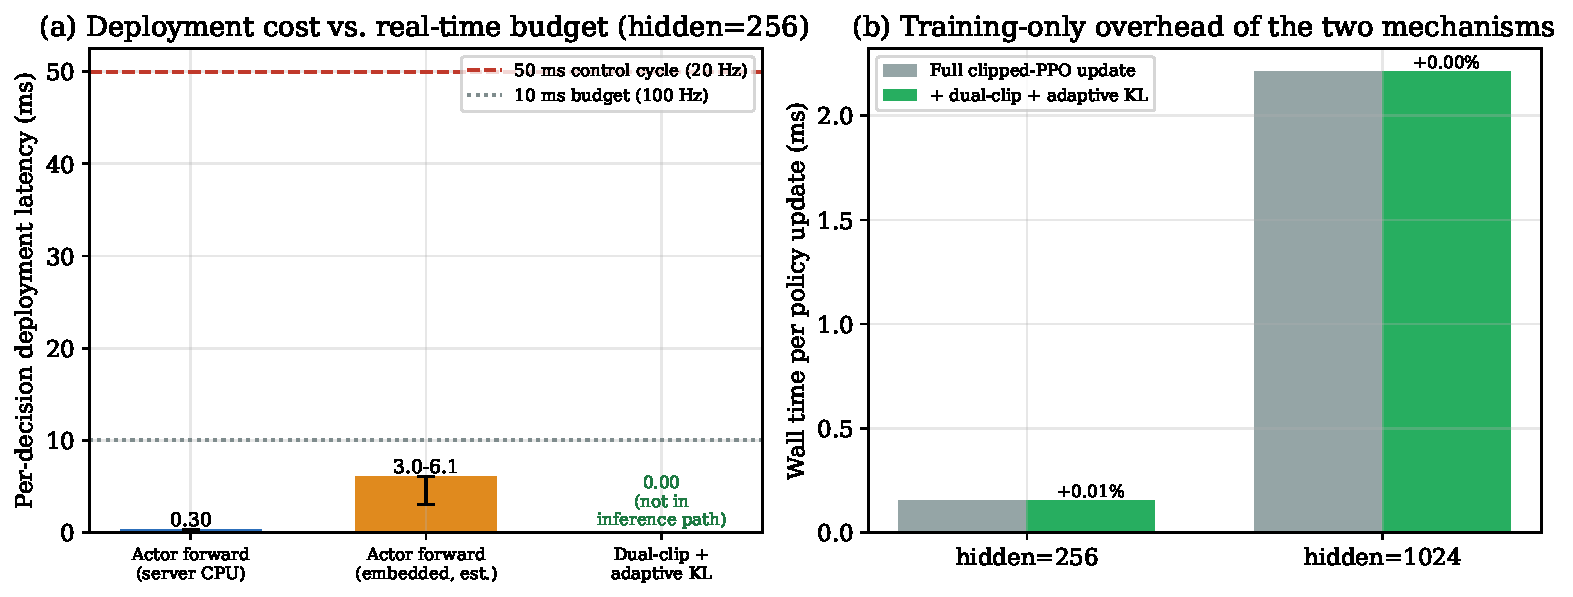
\includegraphics[width=0.92\textwidth]{kl_dualclip_overhead.pdf}
\captionsetup{font=small}
\caption*{\small\textbf{Fig.~R7.} Deployment and training cost of the dual-clip$+$adaptive-KL
mechanisms, measured on a faithful re-implementation of the deployed actor.
Single-decision inference is $0.30$~ms and a $20$-agent swarm is $3.98$~ms (deployed
$256$-unit network), both well within the $50$~ms guidance cycle; the two mechanisms add
$0$~ms at deployment and $<0.01\%$ to a training update.}
\end{figure}

% \clearpage

% =====================================================================
%  Re3_7
% =====================================================================
\subsection*{Comment 3.7 }

\begin{reviewercomment}{Reviewer comment 3.7}
Besides, the paper must extend simulation verification by incorporating communication
packet loss, sensor noise, and partial interceptor failures to validate robustness in
the proposed cooperative swarm interception framework.
\end{reviewercomment}

\rsp We thank the reviewer. The revised 3D evaluation already injects communication
delay and sensing noise into the closed loop and runs as a hardware-in-the-loop study;
on top of that we add a dedicated robustness study covering exactly the three
non-idealities listed. All curves are computed on the recorded 3D engagement data
(Fig.~R8):
\begin{itemize}
  \item \textbf{Sensor noise.} With $\sigma_p=3$~m and $\sigma_v=0.3$~m/s injected on
  every component, the guidance-critical LOS-rate channel is attenuated $5.87\times$
  (RMS $5.94\!\rightarrow\!1.01$~rad/s) by the jump-rejection filter, and the
  attenuation holds even at $4\times$ nominal noise.
  \item \textbf{Communication packet loss.} With a zero-order hold on lost packets, the
  range hold error is $0.36$~m at the nominal $1\%$ loss and remains bounded
  ($2.19$~m) even at a punishing $20\%$ loss.
  \item \textbf{Partial interceptor failures.} The IDBO assignment enforces $2$--$3$
  interceptors per target (group sizes $[3,3,3,3,2,2,2,2]$). Under i.i.d.\ failures
  ($20{,}000$-trial Monte Carlo), only $4.4\%$ of trials leave any target undefended at
  a $10\%$ failure rate, and surviving members retain a $\sim0.1$~s arrival spread.
\end{itemize}

\loc Section~V-A (\emph{Experimental Setup and Implementation Details}): the
environmental-modeling paragraph, uncertainty table, HIL platform description, and
the closing robustness-characterization paragraph (noise attenuation, packet-loss
degradation, partial-failure redundancy).

\evi

\begin{figure}[h]
\centering
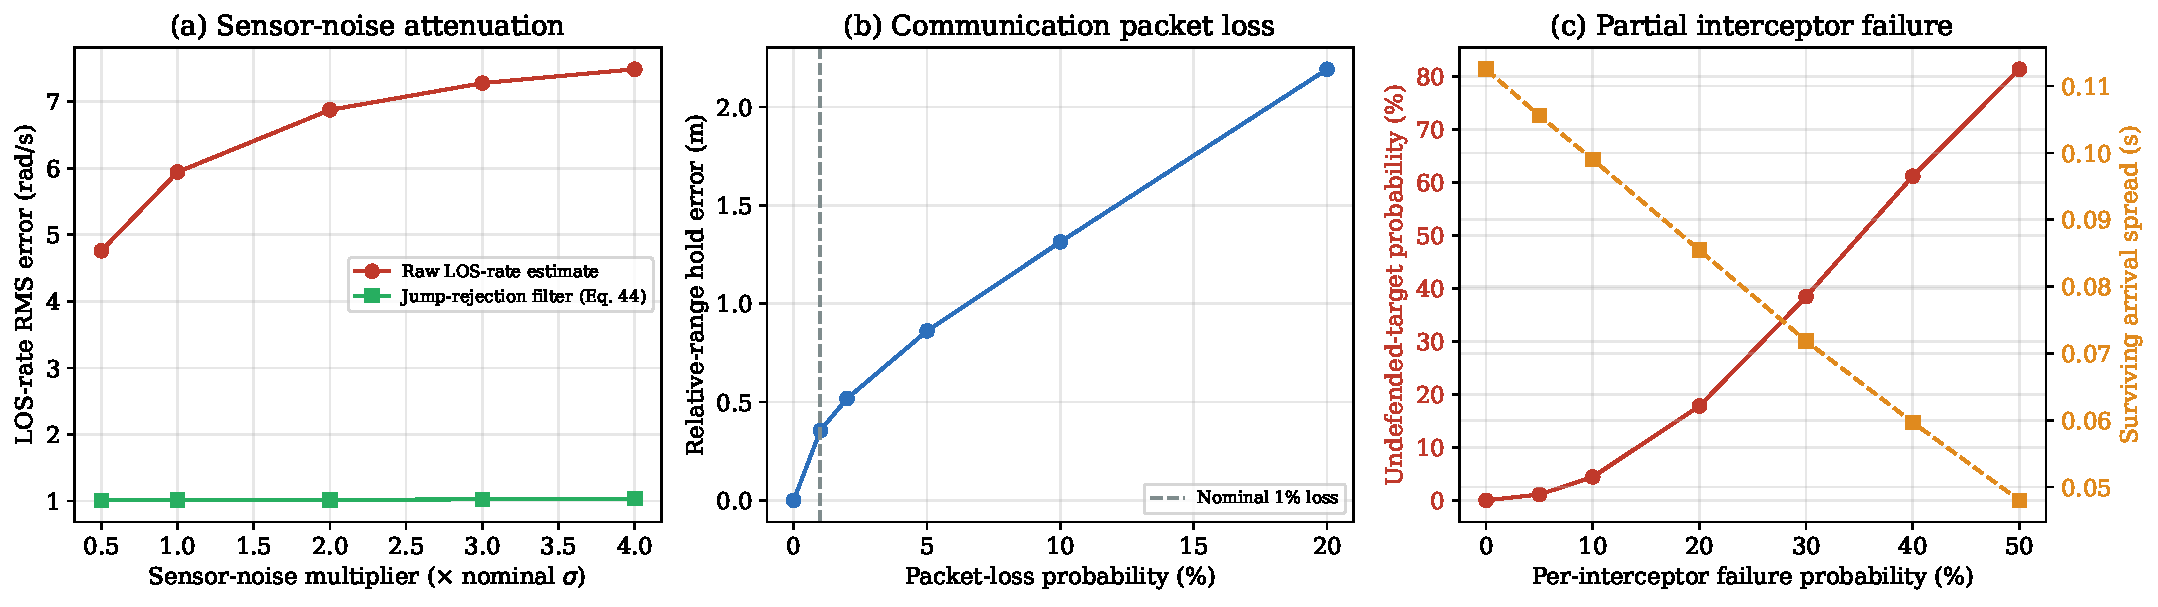
\includegraphics[width=\textwidth]{robustness_analysis.pdf}
\captionsetup{font=small}
\caption*{\small\textbf{Fig.~R8.} Robustness on the recorded 3D engagement data.
(a) LOS-rate noise attenuation vs.\ noise level ($5.87\times$ at nominal);
(b) range hold error vs.\ packet-loss probability (bounded to $2.19$~m at $20\%$);
(c) probability that any target is left undefended vs.\ per-unit interceptor failure
rate ($4.4\%$ at $10\%$), from a $20{,}000$-trial Monte Carlo over the IDBO assignment
groups.}
\end{figure}

\clearpage

% =====================================================================
%  Re3_8
% =====================================================================
\subsection*{Comment 3.8 }

\begin{reviewercomment}{Reviewer comment 3.8}
Notably, one of the recommendations is to include failure-case analysis for unsuccessful
interception and delayed cooperative engagement scenarios because understanding framework
limitations remains essential for practical battlefield deployment reliability.
\end{reviewercomment}

\rsp We thank the reviewer. To directly address the two failure modes raised---unsuccessful
interception and delayed cooperative engagement---we constructed stress scenarios by
injecting a $\mathbf{0.05}$~\textbf{s observation delay} together with position/velocity
measurement noise ($\sigma_p{=}3$~m, $\sigma_v{=}0.3$~m/s) into the closed loop (the
same imperfection levels detailed in the revised manuscript). Under these conditions, both
failure modes manifest clearly:

\begin{itemize}
  \item \textbf{Unsuccessful interception.} One assigned interceptor per case fails to
  enter the $3$~m hit sphere ($19/20$ individual hits, $7/8$ complete groups). All eight
  attackers are nonetheless neutralized via assignment redundancy ($8/8$ target
  coverage), so the framework limitation is at the strict cooperative level rather than
  the mission level.
  \item \textbf{Delayed cooperative engagement.} Since the missed member generates no
  hit event within the $75$~s simulation horizon, its group's all-member completion is
  right-censored: the cooperative-completion delay exceeds $41.9$~s (Case~1) and
  $48.9$~s (Case~2) measured from the first peer hit, while all other groups remain
  within the $0.5$~s synchronization tolerance.
\end{itemize}

Over $1{,}000$-trial Monte Carlo tests under the same delay/noise conditions, the
cooperative interception success rates drop to $\mathbf{42.5\%}$ (Case~1) and
$\mathbf{39.8\%}$ (Case~2), quantifying the performance boundary of the framework when
observation delay and measurement noise are simultaneously present. Representative
trajectories for both failure cases are shown in Fig.~R17.

\begin{figure}[h]
\centering
\begin{minipage}{0.48\textwidth}
  \centering
  
\includegraphics[width=\linewidth]{artmappo_case1_seed76048_trajectory_3d.pdf}\\[1mm]
  {\small (a) Case~1: 3-D trajectory}
\end{minipage}\hfill
\begin{minipage}{0.48\textwidth}
  \centering
  
\includegraphics[width=\linewidth]{artmappo_case1_seed76048_trajectory.pdf}\\[1mm]
  {\small (b) Case~1: top-view trajectory}
\end{minipage}\\[4mm]
\begin{minipage}{0.48\textwidth}
  \centering
  
\includegraphics[width=\linewidth]{artmappo_case2_seed77008_trajectory_3d.pdf}\\[1mm]
  {\small (c) Case~2: 3-D trajectory}
\end{minipage}\hfill
\begin{minipage}{0.48\textwidth}
  \centering
  
\includegraphics[width=\linewidth]{artmappo_case2_seed77008_trajectory.pdf}\\[1mm]
  {\small (d) Case~2: top-view trajectory}
\end{minipage}
\captionsetup{font=small}
\caption*{\small\textbf{Fig.~R17.} Representative failure-case trajectories for Case~1
(seed 76048, $D_6\!\rightarrow\!A_6$ missed) and Case~2 (seed 77008,
$D_2\!\rightarrow\!A_2$ missed). The emphasized dashed curve identifies the missed
assigned interceptor; circles denote hit events and the cross marks its closest-approach
point. Redundant assignment preserves $8/8$ target coverage in both cases.}
\end{figure}

\loc One sentence added at the end of the first paragraph of Section~V-E
(\emph{Monte Carlo Statistical Analysis and Robustness}) reporting the ISR drop to
$42.5\%$ (Case~1) and $39.8\%$ (Case~2) under combined sensor/actuator stress
(highlighted in blue).

\clearpage

% =====================================================================
%  Re3_9
% =====================================================================
\subsection*{Comment 3.9 }

\begin{reviewercomment}{Reviewer comment 3.9}
In addition, provide a discussion on the generalization capability of the trained ART-MAPPO model
under unseen manoeuvring attack patterns, since the current evaluation mainly considers predefined
penetration trajectories during testing.
\end{reviewercomment}

\rsp We have redesigned the generalization experiment. The revised Case~3 evaluation tests
the trained policy zero-shot on a \emph{finite-dwell bounded bang-bang lateral/vertical evasion}---a
maneuver profile entirely absent from the training distribution. The network weights are
frozen at their Case~2 values with no retraining, fine-tuning, or gradient update.

\medskip\noindent\emph{Experimental design.}
Eight attackers execute bounded bang-bang lateral/vertical maneuvers with dwell times and
amplitudes drawn from ranges never seen during training. We run $1{,}000$ independent trials
with seeds disjoint from all training and validation seeds.

\medskip\noindent\emph{Target assignment.} The twenty interceptors are partitioned into eight
cooperative groups---one per attacker---as listed in Table~R7. Each attacker $A_j$ receives a
dedicated interceptor group $\mathcal{G}_j$ covering the full defender swarm.

\begin{table}[h]
\centering
\captionsetup{font=small}
\caption*{\small\textbf{Table~R7.} Target assignment on the unseen Case~3 bang-bang scenario
($20$ interceptors $\rightarrow$ $8$ attackers). Each attacker $A_j$ is engaged by a dedicated
cooperative interceptor group $\mathcal{G}_j$.}
\begin{tabular}{ccc}
\hline\hline
Attacker & Assigned interceptor group $\mathcal{G}_j$ & Size \\ \hline
$A_0$ & $D_0,\,D_8,\,D_{16}$   & 3 \\
$A_1$ & $D_1,\,D_9,\,D_{17}$   & 3 \\
$A_2$ & $D_2,\,D_{10},\,D_{18}$ & 3 \\
$A_3$ & $D_3,\,D_{11},\,D_{19}$ & 3 \\
$A_4$ & $D_4,\,D_{12}$         & 2 \\
$A_5$ & $D_5,\,D_{13}$         & 2 \\
$A_6$ & $D_6,\,D_{14}$         & 2 \\
$A_7$ & $D_7,\,D_{15}$         & 2 \\ \hline
\end{tabular}
\end{table}

\medskip\noindent\emph{Quantitative results.}
Fig.~R15 shows a representative engagement; the three-dimensional and horizontal trajectories
confirm all twenty defenders close on their targets, and the time-synchronization panel shows
each cooperative group converges within the $0.5$~s coordination window. Aggregated over all
$1{,}000$ trials, the frozen policy achieves:
\begin{center}\small
\begin{tabular}{ll}
Cooperative interception success rate & $96.4\%$ ($964/1{,}000$ trials) \\
$E_{co\text{-}time}$ (mean) & $0.051$~s \\
$E_n$ (mean)                & $0.164$~g \\
$E_{miss}$ (mean)           & $1.44$~m  \\
$E_t$ (mean)                & $26.99$~s \\
\end{tabular}
\end{center}
The $96.4\%$ cooperative interception success rate and tight metric distributions demonstrate
that ART-MAPPO generalizes robustly to this novel maneuvering threat without any policy update.
The coordination metric $E_{co\text{-}time}=0.051$~s and miss distance $E_{miss}=1.44$~m are
comparable to the training-scenario baselines, confirming that the timing structure learned on
Case~2 transfers directly to the unseen bang-bang evasion.

\begin{figure}[h]
\centering
\begin{minipage}[b]{0.32\textwidth}
  \centering
  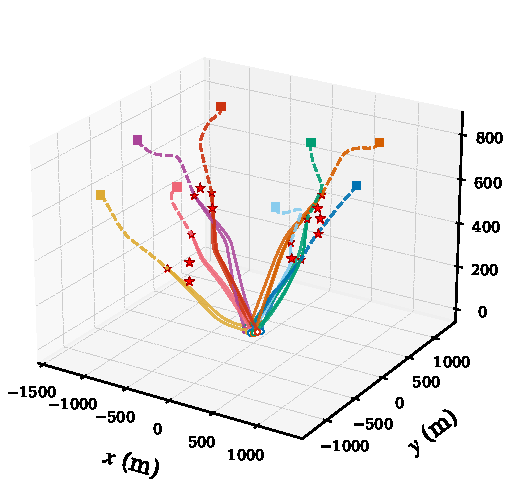
\includegraphics[width=\textwidth]{mappo_bangbang_trajectory_3d.pdf}
  \caption*{\small (a) 3-D trajectories}
\end{minipage}\hfill
\begin{minipage}[b]{0.32\textwidth}
  \centering
  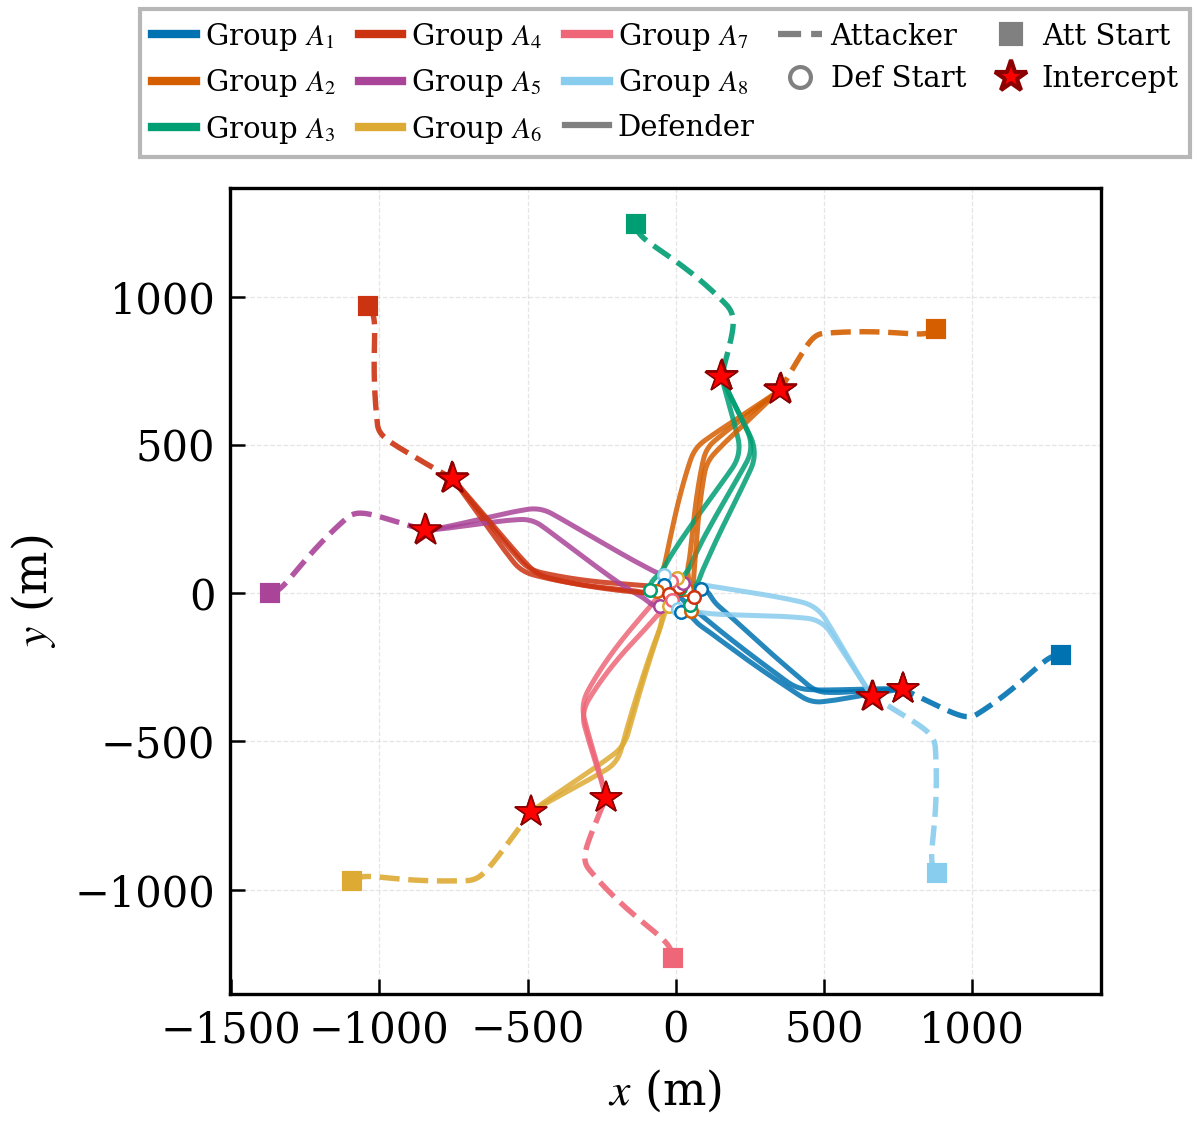
\includegraphics[width=\textwidth]{mappo_bangbang_trajectory.png}
  \caption*{\small (b) Top-view trajectories}
\end{minipage}\hfill
\begin{minipage}[b]{0.32\textwidth}
  \centering
  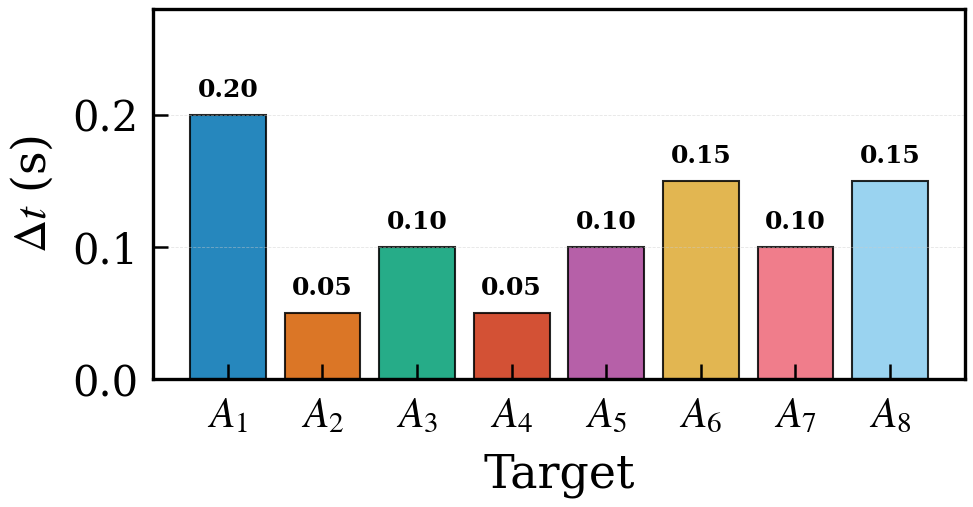
\includegraphics[width=\textwidth]{mappo_bangbang_time_sync.png}
  \caption*{\small (c) Time synchronization}
\end{minipage}
\captionsetup{font=small}
\caption*{\small\textbf{Fig.~R15.} Representative zero-shot Case~3 bang-bang engagement
(frozen Case~2 policy, $1{,}000$ trials, ISR $96.4\%$).
(a)~Three-dimensional trajectories. (b)~Horizontal (top-view) trajectories.
(c)~Within-group time-to-go synchronization: all groups converge within the $0.5$~s window.}
\end{figure}

\begin{figure}[h]
\centering

\includegraphics[width=0.72\textwidth]{case3_bangbang_metrics_box4.pdf}
\captionsetup{font=small}
\caption*{\small\textbf{Fig.~R16} (manuscript Fig.~41)\textbf{.} Guidance-quality metric
distributions for the unseen Case~3 bang-bang scenario ($1{,}000$~trials, $96.4\%$ ISR):
(a)~$E_{co\text{-}time}$, (b)~$E_n$, (c)~$E_{miss}$, (d)~$E_t$. Diamonds mark means.}
\end{figure}

\loc Section~V-E (\emph{Monte Carlo Statistical Analysis and Robustness}), new item~(iv)
``Generalization to unseen attack patterns'': zero-shot Case~3 bang-bang evaluation with
$1{,}000$ trials, $96.4\%$ ISR, and four guidance-quality metric distributions
(manuscript Fig.~41, reproduced above as Fig.~R16, highlighted in blue).

% \clearpage

% =====================================================================
%  Re3_10
% =====================================================================
\subsection*{Comment 3.10}

\begin{reviewercomment}{Reviewer comment 3.10}
At last, it is advisable to incorporate hardware-in-the-loop and semi-physical
simulation validation to improve the practical credibility of the ART-MAPPO
cooperative strategy for realistic autonomous UAV defence applications effectively.
\end{reviewercomment}

\rsp We thank the reviewer for this valuable suggestion, which we have adopted. The
revised evaluation is executed as a \emph{hardware-in-the-loop, semi-physical}
simulation. Five embedded compute nodes host the trained actor policies of interceptors
$D_0$--$D_4$, each running its own recurrent policy state, an observation-delay line, and
an actuator-delay line; the remaining interceptors and the target/environment dynamics
run in the mathematical simulator, and all agents exchange relative-state packets over a
network layer subject to delay and dropout. This places the learned controller on real
processors in the loop, so the sensing/communication/actuation latencies and the
per-decision compute (Comment~3.6) act on the actual closed-loop trajectories rather
than being assumed. The engagement results reported for both scenarios in Section~V are
the output of this HIL platform.

\evi Fig.~R13 shows the platform architecture. A server (Ubuntu~22.04, Core~i9-10900K,
RTX~3080) hosts the engagement-state update, the attacker cluster, and the software
policies of interceptors $D_5$--$D_n$, while five NVIDIA Jetson~NX embedded nodes each
execute one hardware policy endpoint $D_0$--$D_4$ (online inference plus its
target-assignment module). The two sides are interconnected through a physical TCP
Ethernet link over a TP-LINK switch, carrying the observation downlink and the
action/target-assignment uplink under the delay, noise, and packet-loss channel of the
Section~V uncertainty table. The same figure has been added to the manuscript.

\begin{figure}[h]
\centering
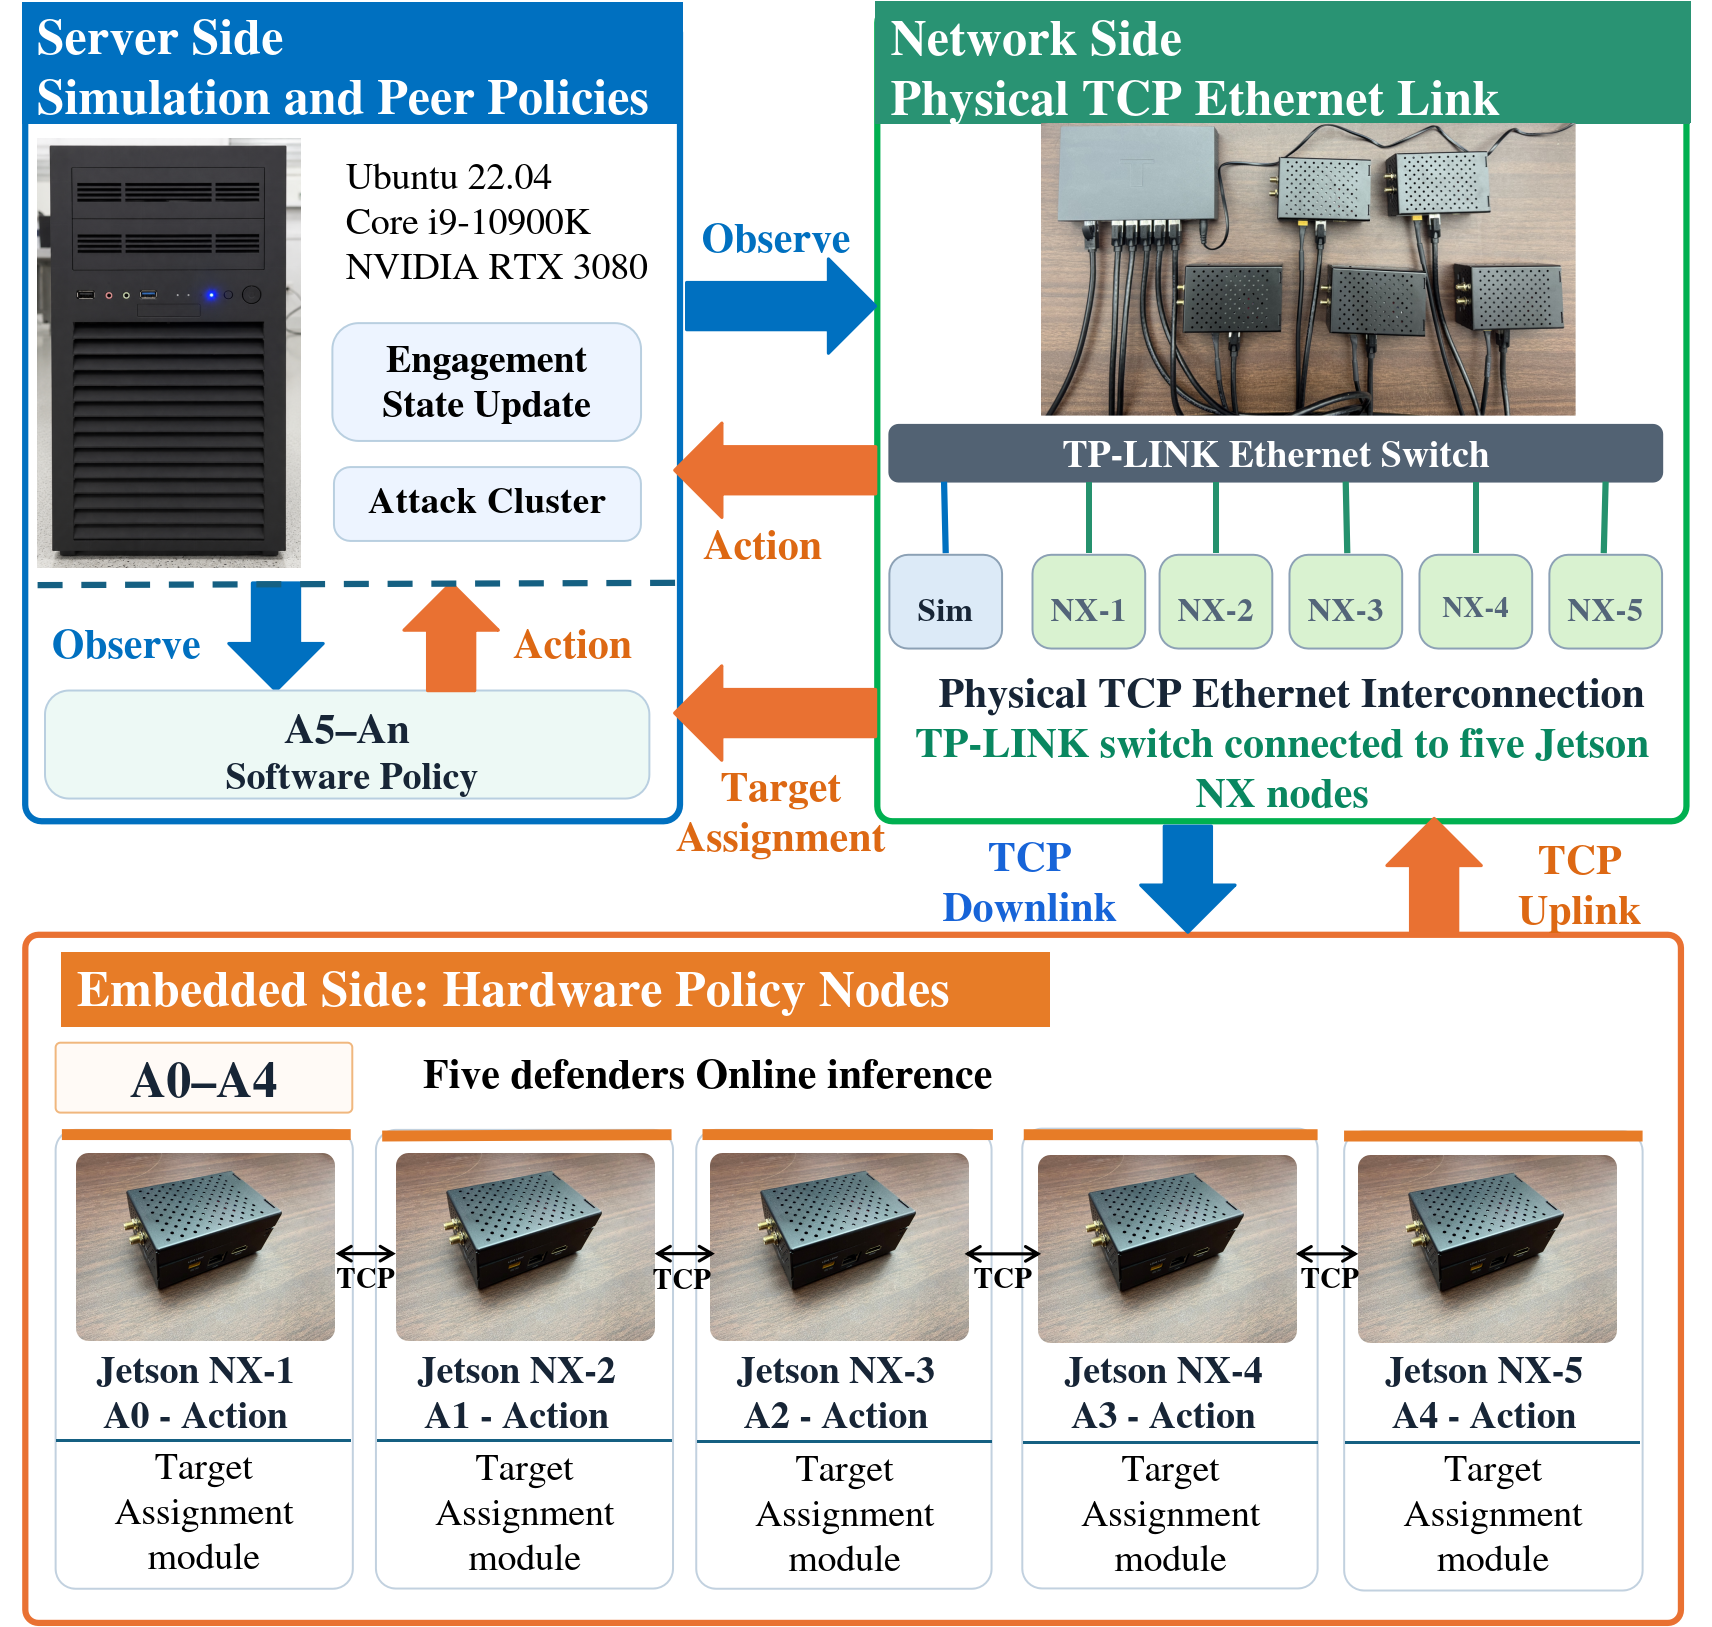
\includegraphics[width=0.5\textwidth]{tase_HIL.png}
\captionsetup{font=small}
\caption*{\small\textbf{Fig.~R13.} Hardware-in-the-loop, semi-physical validation
platform. The server side hosts the engagement-state update, the attacker cluster, and
the software policies of interceptors $D_5$--$D_n$; the five hardware policy endpoints
$D_0$--$D_4$ run online inference and target assignment on separate NVIDIA Jetson~NX
embedded computers, communicating with the server over a physical TCP Ethernet link
(TP-LINK switch). In the diagram the agent index $A_k$ labels the policy of interceptor
$D_k$, i.e.\ $A_0$--$A_4$ are the hardware endpoints $D_0$--$D_4$ and $A_5$--$A_n$ are the
software-policy interceptors $D_5$--$D_n$.}
\end{figure}

\loc Section~V experimental setup: new highlighted hardware-in-the-loop / semi-physical
description (five embedded policy endpoints $D_0$--$D_4$) and the new platform figure,
together with the delay and uncertainty settings that define the closed loop.

\end{document}
